\documentclass[12pt]{article}
\usepackage{graphicx}
\graphicspath{ {./images/} }
\usepackage{placeins}
\usepackage{hyperref}
\usepackage{array}
\usepackage{wrapfig}

\title{ShipCAD manual\\Version 2.6}
\author{Greg Green}

\begin{document}

\maketitle

\begin{center}
\begin{tabular}{ m{8cm} m{5cm} }
Homepage & www.freeship.org \\
ShipCAD project page & \url http://sourceforge.net/projects/freeship \\
Contact & info@freeship.org \\
Send designs for the database to & designs@freeship.org
\end{tabular}
\end{center}
Copyright © 2005, 2006 by M. v. Engeland

\section{Contents}

\tableofcontents
\pagebreak

\section{ShipCAD}

This manual is distributed as part of the ShipCAD project.

ShipCAD is an open source surface-modeling program based on
subdivision surfaces and intended for the design of ships.

The program is free software; you can redistribute it and/or modify it
under the terms of the GNU General Public License as published by the
Free Software Foundation; either version 2 of the License, or (at your
option) any later version.

The program and manual are distributed in the hope that it will be
useful, but WITHOUT ANY WARRANTY; without even the implied warranty of
MERCHANTABILITY or FITNESS FOR A PARTICULAR PURPOSE. See the GNU
General Public License for more details, as enclosed at the end of
this manual.

You should have received a copy of the GNU General Public License
along with this manual.  if not, write to:

The Free Software Foundation, Inc.,
59 Temple Place, Suite 330
Boston, MA 02111-1307
USA

Special thanks to:
\begin{itemize}
  \item Paul Unterweiser for creating the website
  \item Stefan Probst for his continuing support, advice, patience and developing the script
used for the online database.
  \item John Winters for help regarding the KAPER resistance method.
  \item Leo Lazauskas for adapting Michlet and answering numerous questions.
  \item Alain Bertrand for testing ShipCAD under different window managers under WINE
  \item Antoine Birckel for translating the manual into French
  \item Andrey Factor and Bruce Taylor for repeatedly beta testing new features as well as
their constructive comments.
\end{itemize}

\section{ShipCAD and Linux.}

Free!ship is originally intended for Windows, although users have
reported that it runs rather well under WINE too. In some cases
problems might be experienced with the window focus. In Windows the
dialog that has focus always stays in front of the mainform. Under
Wine the dialog windows of ShipCAD go sometimes to the background
while retaining user input focus. As a result, ShipCAD seems to be
crashed while it hasn't. To solve this problem, you must cycle through
the windows to get the dialog window back to the foreground and close
it. Unfortunately, some window managers don't allow this because not
all of the open windows are listed in the window menu. The following
are the results of some tests that have been done on a Ubuntu Breezy
Badger.  KDE 3.5 Unusable. The menus don't stay opened so no menu item
can be chosen.  Gnome Only the main window of ShipCAD is listed in the
window menu, so if you loose the focus of a dialog window, your only
choice is to kill ShipCAD.  Fluxbox OK IceWm OK WindowMaker OK Openbox
OK Blackbox Not tested, but as Blackbox is quite close to Fluxbox it
is probably ok.

\pagebreak

\section {Introduction.}
ShipCAD uses a technique called surface modeling to define the shape
of a ship. This technique involves “sculpting” the hull as if it were
a very thin and flexible piece of cloth by pulling and shifting
points. It is however not limited to the hull alone as we will see
later. Decks, superstructures, masts, keels and rudders can be modeled
this way too. Unlike other programs, ShipCAD uses subdivision surfaces
to completely model the ship. Subdivision surfaces give the designer
more flexibility in designing any desired shape. But when you want to
get the most of this technique it is important to have a basic
understanding of some of its underlying principles. An example of the
hull a simple demo yacht can be seen on Figure \ref{fig:mesh}. The
actual surface is a mesh consisting of the following 3 objects:

\begin{itemize}
  \item Faces
  \item Edges
  \item Points
\end{itemize}

\begin{figure}[h]
        \centering
        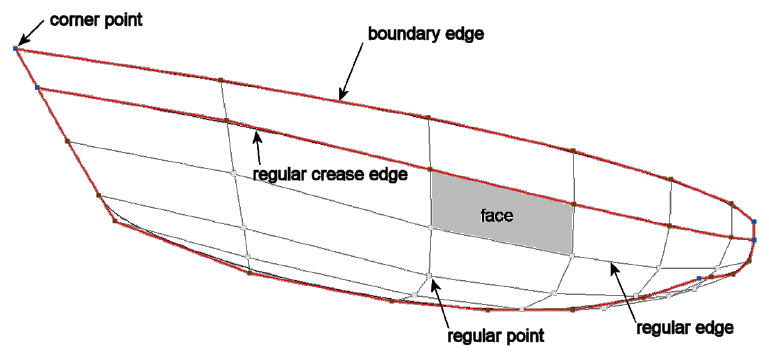
\includegraphics[width=15cm,natwidth=769,natheight=355]{figure1.png}
        \caption{}
        \label{fig:mesh}
\end{figure}

\subsection{Faces.}
A face is a little piece of the entire surface (sometimes also called
a patch) and is usually defined with 4 points.\par In some areas it is
desirable to have less (or even more) points, but generally the best
results are obtained when most of the faces consist of 4 points.

\subsection{Edges.}
All successive points of the face are connected by lines. These lines
are called edges and can be divided into two different kinds of edges.

\begin{itemize}

  \item \textit{Boundary edges}. These are edges which form, as the
  name suggests, the boundary of the surface. A boundary edge is
  characterized by the fact that it has \textbf{always}
  only \underline{\textbf{1}} face attached to it. Examples of
  boundary-edges are the sheer line (when the ship is not fitted with
  a deck) or the centerline of the ship. The centerline, or profile,
  is in fact a special case.  When defining the hull only its portside
  is created. So all edges on the center plane are boundary-edges as
  they have only one face connected to it. In reality the ship is
  symmetric, and when performing calculations ShipCAD creates a
  virtual symmetric ship by mirroring the model in the center plane.

  \item \textit{Regular edges}. These are all other edges away from
  the boundary of the surface, and must \textbf{always} be shared
  by \underline{\textbf{2}} adjacent faces. Regular edges are drawn as
  dark-gray lines. The two faces connected to an edge are joined
  smoothly along their shared edge. It is possible however to mark an
  edge as a crease-edge. When doing so, the two faces are joined in a
  tangent-discontinuous way. In other words, crease-edges are used to
  define knuckle lines. A boundary-edge is in fact a specific case of
  a crease edge since there is no second face to make a smooth
  transition.

\end{itemize}

ShipCAD uses the presence of boundary-edges in its calculations. By
doing so it is able to determine when the ship is making water when
for example the deck line is submerged. The downside to this is that
it is critical for any regular edge to be connected to two faces, at
least when not submerged. Having two different edges which are located
precisely on top of each other is not sufficient. Faces have to be
physically connected to the \textbf{same} edge. There is also another
reason for this which will be explained
in \ref{guidelines}. Boundary-edges from which both the startpoint and
endpoint are located on the center plane are excluded from this test.
In reality these edges are connected to both the portside and the
starboard side of the ship and are therefore not truly a
boundary-edge.

\subsection{Points.}
Points form the basis of the surface. Most of the editing is done on a point-level by moving points to
different locations, inserting new points or removing existing points. Basically there are two different
types of points of interest to the user. These are:

\begin{itemize}
  \item Regular points. These are all points other then cornerpoints. It is important to realize that
these points have a certain offset to the resulting surface. This deviation to the surface is
bigger in surface areas with high curvature. It becomes less when more points and edges
are inserted.
  \item Cornerpoints. Cornerpoints are specific points, usually connected to 2 or more crease-
edges. Just like a crease-edge can be used to specify that two faces have to be connected
in a discontinuous way, cornerpoints may be used to do so with two adjacent edges.
Cornerpoints are the only type of points actually located on the hull surface. Points where 3
or more crease-edges meet are automatically set to cornerpoints by the program.
\end{itemize}

\subsection{Subdivision surfaces.}

A subdivision surface is a special type of spline-surface. Normally
modeling programs work with parametric spline surfaces like B-Spline
surfaces or NURB surfaces. These surfaces are completely described by
a set of controlpoints.

\begin{wrapfigure}{l}{0.3\textwidth}
        \centering
        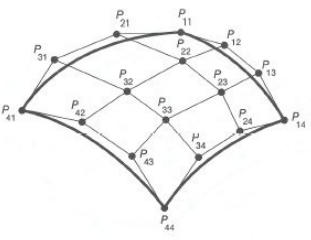
\includegraphics[width=0.3\textwidth,natwidth=311,natheight=240]{figure2.png}
        \caption{}
        \label{fig:mesh1}
\end{wrapfigure}

Controlpoints are the points which the user can modify to control the
shape of the surface. Any point on the surface can be calculated from
these controlpoints using a set of parametric formulas. The drawback
of these parametric surfaces is that they always require a
“rectangular” grid of controlpoints. These controlpoints in reality
might follow the shape of a hull, so they do not look like a true
rectangular grid. But they always have say \textit{\textbf{N}} points
in the longitudinal direction and \textit{\textbf{M}} points in the
vertical direction where both N and M might be any number equal to or
larger than 2. In the figure left \textit{\textbf{N}}=4
and \textit{\textbf{M}}=4 and the number of controlpoints equals
4*4=16. With parametric spline surfaces it is not possible to insert a
single new point on an edge. Instead an entire row of points have to
be inserted as demonstrated in the figure to the right.

\begin{wrapfigure}{r}{0.3\textwidth}
        \centering
        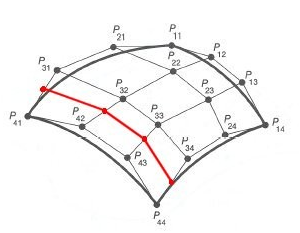
\includegraphics[width=0.3\textwidth,natwidth=300,natheight=233]{figure3.png}
        \caption{}
        \label{fig:mesh2}
\end{wrapfigure}

This results in having more controlpoints than actually needed or
desired, and more controlpoints mean more work to the designer. Also
very complex shapes cannot be modeled using only one surface. When
using multiple surfaces the designer is challenged with the difficult
task of aligning these surfaces at their boundaries. It is often
desirable to maintain a smooth transition along these boundaries. Each
time one of these surfaces is modified, the other surface has to be
modified by the user to maintain this smooth transition.

To overcome these problems ShipCAD makes use of subdivision
surfaces. Subdivision surfaces also use controlpoints as a modeling
handle, just like NURBS or B-Splines. With subdivision surfaces the
grid of controlpoints does not need to be rectangular, but calculating
a point on the surface is more difficult since the surface is not
parametric. Instead the controlmesh is refined and smoothed in a
number of steps. Each step is called a “subdivision step”, hence the
name subdivision surfaces. This process is clarified in
Figure \ref{fig:mesh3}:

\begin{figure}[h]
        \centering
        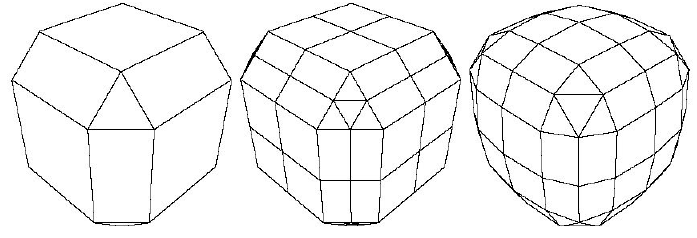
\includegraphics[width=15cm,natwidth=697,natheight=238]{figure4.png}
        \caption{}
        \label{fig:mesh3}
\end{figure}

To the left the controlmesh of a beveled cube is visible. The first
step in the subdivision process is refining the mesh. This is done by
inserting a new point on each edge (called an edge-point).  Whenever a
new edge-point is calculated, information from both adjacent faces is
retrieved. This is another reason why edges always must be shared by
two faces. For each face which has four points or more a point is also
inserted at the center of each face (called a face-point). For faces
with three points each new edge-point is connected with the new point
of the previous edge, thus creating 4 new triangles. All other faces
are subdivided by connecting each edge-point to the face- point. This
way a refined mesh is created which still has the same shape as the
original. This is shown in the middle. Finally all the points in the
surface are shifted to a new location in such a way that the surface
appears smooth. This is called averaging in subdivision terms (right
side). If this process is repeated a number of times a very fine and
smooth mesh is the result. ShipCAD shows a dropdown box in the toolbar
showing the precision of the model. This is actually a measure for how
many subsequent subdivision steps the program performs.

\begin{figure}[h]
        \centering
        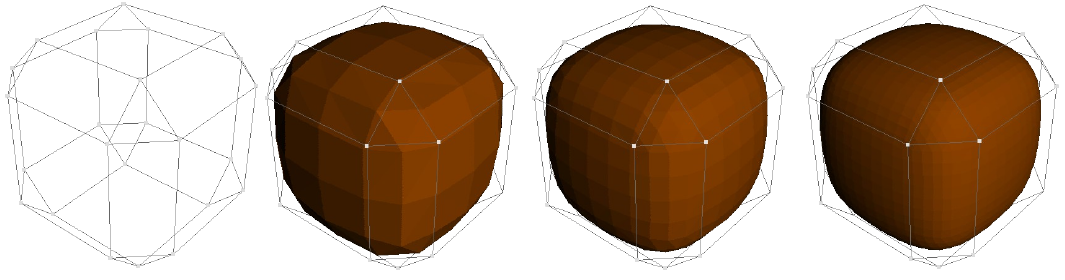
\includegraphics[width=12cm,natwidth=1065,natheight=280]{figure5.png}
        \caption{}
        \label{fig:mesh4}
\end{figure}

Figure \ref{fig:mesh4} shows the controlmesh of the same beveled cube
and the resulting surface after 1, 2 and 3 subdivision steps is shown.

\begin{figure}[h]
        \centering
        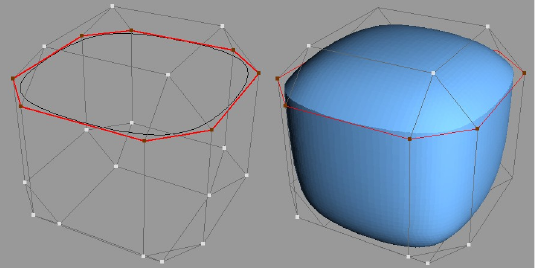
\includegraphics[width=15cm,natwidth=535,natheight=268]{figure6.png}
        \caption{}
        \label{fig:mesh5}
\end{figure}

This is the same cube, but a number of edges have been marked as
crease-edges (red lines). The result is a sharp knuckle line going
around the cube. It is clearly visible that faces adjacent to the
crease-edges are no longer joined in a smooth manner.
\pagebreak

\subsection{Guidelines to subdivision modeling.} \label{guidelines}
In this paragraph some guidelines are given to obtain the best
results.

\begin{itemize}

\item Use a regular grid whenever possible. A grid is considered
regular if all faces consist of four points, and all points are
connected to four edges and faces. A point on the boundary is
considered regular if it has 3 edges and two faces connected to
it. Off course this is not always possible.  Triangular faces may be
used as a means to reduce the number of points in an area.  5-sided
faces, or 5 4-sided faces can be used to increase the number of
points. A truly regular grid would look exactly as the B-spline
surface in the previous paragraph.

\begin{figure}[h]
        \centering
        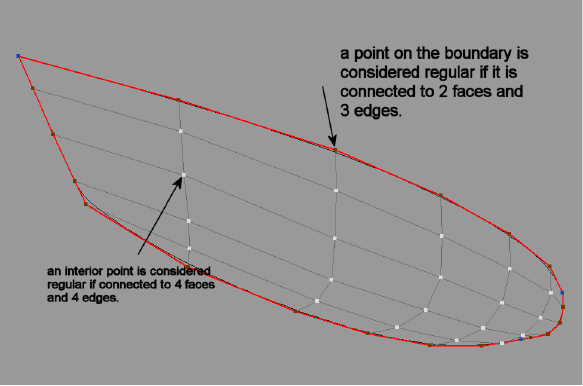
\includegraphics[width=5cm,natwidth=583,natheight=386]{figure7.png}
        \caption{}
        \label{fig:mesh6}
\end{figure}


  \item Whenever possible always have two faces connected to all edges
other than boundary-edges. If more than two edges are connected to an
edge, that specific edge will be drawn thicker and in a light green
color. This must be avoided at all cost as it messes up hydrostatic
calculations. Boundary-edges are allowed, but as soon as they become
submerged hydrostatics will not be calculated anymore. See also \ref{check-model}.

  \item Make sure that the normals of all the faces point outward (in
the direction of the water). This is of uttermost importance since
ShipCAD calculates hydrostatics by integrating the enclosed
volume \textbf{at the back} of the faces. If the normal of a face
points inward, the volume \textbf{outside} the hull would be
calculated and might even become negative. By using the actual surface
for hydrostatic calculations instead of a number of stations, a higher
accuracy is obtained. This is especially true when the model has a
heeling angle and/or trim, or is fitted with a superstructure. ShipCAD
can also check the direction of normals automatically, but correctness
is only guaranteed if the model is totally closed, meaning that no
other boundary-edges are present except the edges lying on the center
plane. Automatic checking can be disabled in the project settings
dialog as explained in \ref{project-settings}.

\end{itemize}

\pagebreak

\section{Viewports.}

\subsection{Zooming and panning.}

\begin{wrapfigure}{r}{0.4\textwidth}
        \centering
        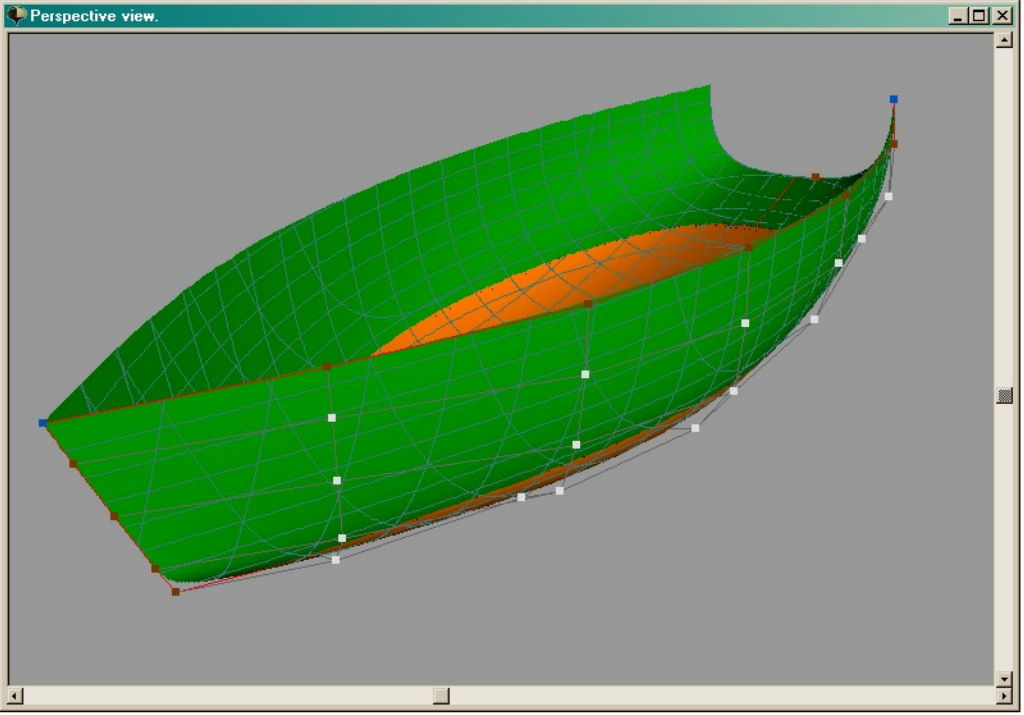
\includegraphics[width=0.4\textwidth,natwidth=1024,natheight=715]{figure8.png}
        \caption{}
        \label{fig:viewport}
\end{wrapfigure}

When a new model is opened or started the program by default adds 4
windows. Each window has a different view on the 3D hull. The area of
the window on which the model is drawn is called a viewport. Zooming
in or out on the viewport is done by pressing the left mouse button
and moving the mouse up or down while keeping the left button pressed.
Users having a mouse wheel may find it convenient to zoom in or out
using their mouse wheel. Panning the viewport is done in a similar
manner, only with the right mouse button must be pressed. Only when
the viewport displays a perspective view, as in the image to the
right, two scrollbars are visible. These can be used to rotate and
tilt the model. Another way to rotate the model is keeping the middle
mouse button (or mouse wheel) pressed while dragging the mouse, also
only in a in a perspective view. Additional options for each viewport
are accessible from the popup-menu which shows after the right button
of the mouse has been pressed.

\subsection{Selecting items.}
Only items visible in the viewport can be selected and only if the
viewport is in wireframe mode (shading is turned off). In order to
select points or edges the Control Net has to be
turned on. Faces can only be selected when
the interior edges are turned on. For more
information concerning visibility options the reader is referred
to \ref{visibility-options}. It is important to keep in mind that
selected faces, edges or points remain selected even when they are not
visible in the viewport due to a change in the visibility options. To
select an item, simply click on it with the mouse. Selected items can
be recognized because they are drawn in yellow. If a point is
selected, and the user clicks on a different point, this new point
will be selected and the previous point will be deselected.  Selecting
multiple points however is possible by keeping the CTRL-key pressed
while clicking on a new point.

If the CTRL key is pressed while an edge is being selected, the
program tries to trace the edge until a irregular point is encountered
or an edge with a different crease-property. This way it is easy to
select an entire row of edges (edgeloop) such as for example the
sheerline or a hard chine.  Faces also can be CTRL-selected. In that
case all the faces belonging to the same layer and connected to the
selected one are also selected or deselected. Faces that are isolated
from the selected face because they are totally surrounded by crease
edges are not included.

\subsection{Dragging control points.}
One of the most important options when it comes to modeling the hull
is dragging points. In order to do this the controlnet must be turned
on. Although it is possible to select points in a perspective view,
the actual dragging of the point can only be done in the bodyplan
view, profile view or plan view. When dragging a controlpoint all
information is updated realtime. This includes stations, buttocks,
waterlines and diagonals. Especially when the precision of the model
is set to a high value this updating might become slow since each
intersection with the hull must be recalculated. If it becomes too
slow, try using a lower precision. If it is still too slow, switch off
some of these intersection curves since only visible items are
recalculated, or try using less intersection curves.

\begin{wrapfigure}{r}{0.2\textwidth}
        \centering
        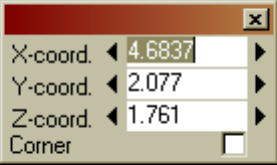
\includegraphics[width=0.2\textwidth,natwidth=277,natheight=165]{pointdialog.png}
        \caption{}
        \label{fig:pointdialog}
\end{wrapfigure}

\subsection{Modifying controlpoints manually.}
If a point is selected, the form displayed to the right is shown, and
the position of the point in 3D-space is displayed in it. These values
can be altered manually by typing the new location in the appropriate
fields. In addition to that the values can also be altered relatively
to the current location by typing the character @ in front of the
numerical part. If for example the string @-0.2 is entered in the
field for the y-coordinate, then all the y-coordinates of \textbf{all}
selected points will be decreased by 0.20. So the y-coordinate for the
displayed point becomes 2.10-0.20=1.90. This is a convenient way to
shift a number of selected points. If the project uses imperial units
then it is also possible to enter a feet-inch/8 value as follows:
3-2-1, meaning 3ft 2 1/8 inch.

Another way of moving points is by
pressing the arrow keys in the bodyplan, profile or plan view.  The
active point moves a certain distance in the direction of the arrow
key that was pressed. This distance, called “incremental distance” is
visible at the statusbar of the program, next to the amount of undo
memory that is in use. If clicked on the text displaying the
incremental distance a dialog appears in which a new value for the
incremental distance can be specified. Another and faster way is to
press either the + or – key. The incremental distance is then changed
by 10\%.

The black arrows displayed next to each input field on the
controlpoint form can be used to increment the values with the same
incremental distance as mentioned above.

\begin{wrapfigure}{r}{0.3\textwidth}
        \centering
        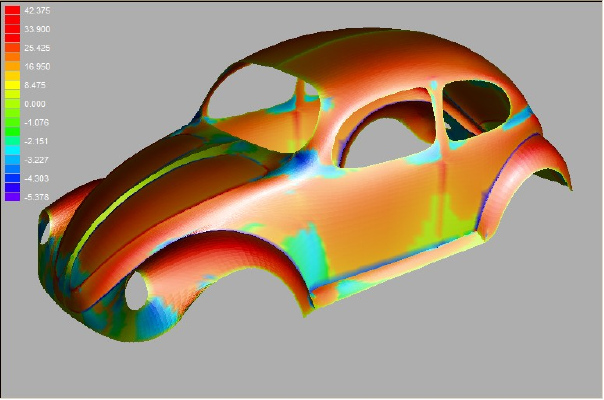
\includegraphics[width=0.3\textwidth,natwidth=604,natheight=400]{surfacecurvaturevw.png}
        \caption{}
        \label{fig:surfcurvvw}
\end{wrapfigure}

\subsection{Different drawing modes.}
ShipCAD has three different drawing modes which are accessible from the popup-menu under the
right mouse button.

\begin{itemize}

  \item Wireframe (Ctrl-W). Only the points, lines and edges are drawn.

  \item Shade (Ctrl-F). The surfaces are drawn in a solid color, lines
are drawn on top of it. The submerged part of the surface can
optionally be shown in a different color.

  \item Developability check (Ctrl-D). The surfaces are shaded again,
only this time parts that are developable are shaded green and parts
that are not developable are shaded red. More about developable
surfaces can be found in \ref{layer-properties} dialog
and \ref{develop-plates}.

  \item Gaussian curvature (Ctrl-G), used to check the fairness of a
surface. The model is shaded in colors, based on the discrete Gaussian
curvature in each point. Most hulls are curved in two directions,
called the principal curvatures.  Gaussian curvature is the product of
these two principal curvatures. Now there are 3 possibilities here:

  \begin{itemize}

    \item \textbf{Negative Gaussian curvature}. These areas are shaded blue and
have the shape of a saddle, since the curvature in one direction is
positive while the curvature in the other must be negative.

    \item \textbf{Zero Gaussian curvature}. At least one of the two principal
curvatures is zero, so the surface is either flat or curved in only
one direction. In both cases the surface is developable (This is in
fact a very important property of developable surfaces). These areas
are shaded green.

    \item \textbf{Positive Gaussian curvature}. The curvature in both
directions can be positive or negative, but must have the same
sign. These areas are convex or concave and shaded red.

  \end{itemize}

\begin{wrapfigure}{r}{0.3\textwidth}
        \centering
        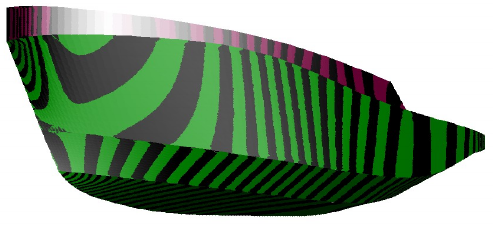
\includegraphics[width=0.3\textwidth,natwidth=493,natheight=233]{zebrashading.png}
        \caption{}
        \label{fig:zebra}
\end{wrapfigure}

  \item Zebra shading (Ctrl-E). Another option to check the model for
fairness. Regions with a constant light-reflection intensity are
shaded in bands. This is similar to the way the human eye detects
unfair spots on a surface since the shininess and shadows vary in
those areas. If the edges of the zebra stripes are curved smoothly
then the surface is smooth in these areas. At knuckle lines they vary
abrubtly.

\end{itemize}

\subsection{Printing.}
Viewports can be printed, but only if they are in wireframe
mode. Regardless of the zoom state of the viewport, the entire model
will be send to the printer. If the current view is a perspective view
then the scale of the print will be such that the model fits the
paper. Other views may be printed to scale.

\begin{wrapfigure}{r}{0.3\textwidth}
        \centering
        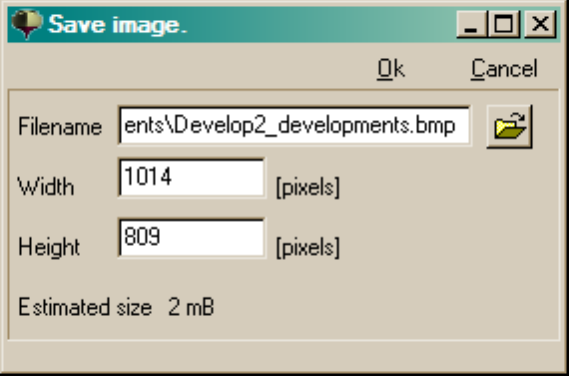
\includegraphics[width=0.3\textwidth,natwidth=570,natheight=377]{saveimagedialog.png}
        \caption{}
        \label{fig:saveas}
\end{wrapfigure}

\subsection{Save as bitmap image.}
The image as shown in the viewport can also be saved to disk. The
following dialog appears in which the desired width or height might be
specified. It is also possible to enter the filename and the file
location.

\pagebreak

\section{File menu.}
From the file menu various options are available.

\subsection{New.}
This starts a new model. The following dialog is shown:

\begin{wrapfigure}{r}{0.3\textwidth}
        \centering
        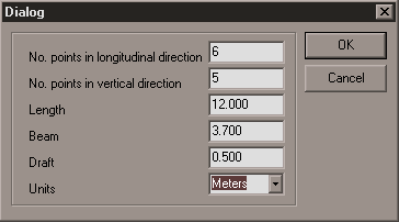
\includegraphics[width=0.3\textwidth,natwidth=401,natheight=223]{filenewdialog.png}
        \caption{}
        \label{fig:filenew}
\end{wrapfigure}

The number of points in longitudinal direction means how many
“columns” of points are desired. Points on these columns are roughly
in the ordinate plane.  The number of points in vertical direction
means the number of points on each “column” from the bottom up. The
desired number of points depends on (and Illustration 9 increases
with) the complexity of the final hull. But it is easier to obtain a
fair surface when the number of points is kept as low as
possible. Also the amount of work is reduced, since fewer points have
to be faired. Extra points might always be inserted later on in the
process, especially in surface areas with high curvature (such as the
bilge or bulb). The input values for length and draft speak for
itself. With beam is meant the total moulded beam. The last option
enables to user to switch between metric units (meters) or imperial
units (feet and inches).

\subsection{Open.}
Use the open option to read an existing ShipCAD model from
file. Starting with version 1.90 ShipCAD saves files to a new binary
format with the .fbm extension. The old files with the .free extension
can still be imported, but saving of this format is no longer
supported. Files can still be transferred to older version of the
program by using the .fef import/export. To open a .free file, click
the open command in the mainmenu. When the opendialog appears, select
``Old freeship files (*.free)'' from the dropdownbox at the bottom of
the dialog.

\subsection{Save.}
This option saves the current model to file. If a file is saved and a
file with that name already exists, it is renamed by changing the
extension from \textit{.fbm} to \textit{.bak} This way a backup file is created.

\subsection{Save as.}
Save the model while prompting for a filename.

\subsection{Import.}
FREE!Ship imports the following file formats:

\subsubsection{Part.}
You can import a part file and add it to the present geometry. How to
create part files is discussed in \ref{part}. ShipCAD automatically
detects if the part file uses imperial or metric units and scales the
imported geometry to suit the type of units used for the current
project.

\begin{wrapfigure}{r}{0.3\textwidth}
        \centering
        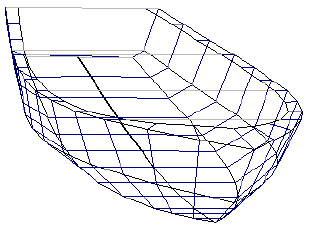
\includegraphics[width=0.3\textwidth,natwidth=311,natheight=229]{filecarlson.png}
        \caption{}
        \label{fig:carlson}
\end{wrapfigure}

\subsubsection{Carlson .hul file.}
Import files created with Carlson Hulls shareware program, which is
available from
\url{http://www.carlsondesign.com/hulls.zip}. Information about the rig will not be imported. When
importing a file, the user may specify if the intermediate bulkheads, as specified in Hulls, should
also be imported. If not then only 5 points on each subsequent chine are imported. From version
1.90 and up a new spline is fitted through the points defined in
the Hulls program. Although the actual points in ShipCAD are
still outside the hull the points as read from th .hul file are
exactly on the hull. This can be easily checked because the
original chines from the file are imported and added to the
model as markers. Controlcurves are added to the crease
edges corresponding to each chine which should coincide with
the markers.
Illustration 10

\subsubsection{Import .fef file.} \label{import-fef}
The Fef file format
(\textbf{F}REE!ship \textbf{E}xchange \textbf{F}ormat) is of no
interest to most users since it mainly supported by other programs
from the same developer.

\begin{wrapfigure}{r}{0.4\textwidth}
        \centering
        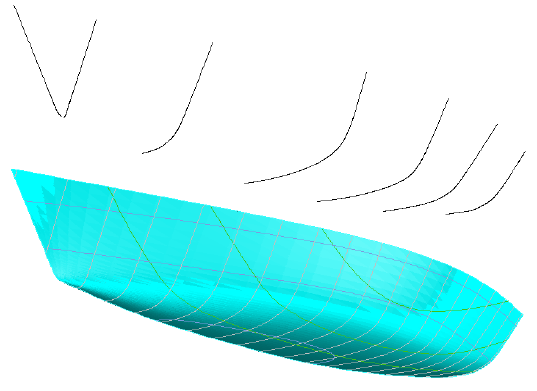
\includegraphics[width=0.4\textwidth,natwidth=537,natheight=391]{filesurface.png}
        \caption{}
        \label{fig:filesurface}
\end{wrapfigure}

\subsubsection{Surface.} \label{import-surface}
Import a textfile containing a number of 3D curves. This option can
best be used when the offsets of a round bottomed hull need to be
imported. These curves may have any number of points which may differ
from curve to curve. Usually the curves run from the bottom of the
hull upwards, however longitudinal curves are allowed too, just as
long as all the curves have the same orientation and run in the same
direction. It is important that the curves are \textbf{not} crossing
each other.

\begin{wrapfigure}{l}{0.4\textwidth}
        \centering
        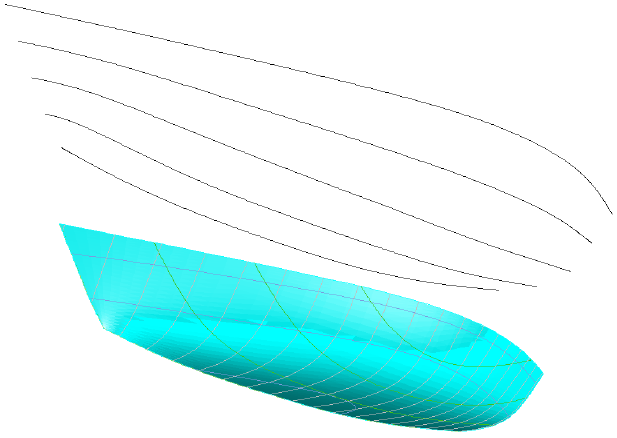
\includegraphics[width=0.4\textwidth,natwidth=617,natheight=438]{filesurfacewaterline.png}
        \caption{}
        \label{fig:filesurfacewaterline}
\end{wrapfigure}

The user will be prompted how many points in longitudinal direction
(number of columns) and in vertical direction (number of rows) the
imported hull must have. Then the program fits a B-Spline surface
through these points such that the new surface interpolates these
points.

The first line of the file must either be a 0 (zero) or a 1. A zero
indicates that all coordinates are in meters while a one indicates
that the coordinates are in feet. Each curve is defined by a sequence
of X,Y and Z coordinates separated by at least 1 space. The end of a
curve is indicated by an empty line after the last coordinate. The
last line in the file should be 'EOF'. The following is an example of
a file containing 3 stations.

\begin{verbatim}
0 
10.62990 0.00000 1.75504 
10.62990 0.15186 1.87085 
10.62990 0.36387 2.07768 
10.62990 0.51880 2.25144
10.62990 0.71454 2.51209 
10.62990 0.91032 2.83897 
10.62990 1.03680 3.13278 
10.62990 1.10212 3.33143 
10.62990 1.18380 3.65010 
11.81100 0.00000 2.26416 
11.81100 0.20519 2.48343 
11.81100 0.36424 2.71927 
11.81100 0.55190 3.09169 
11.81100 0.68655 3.41447 
11.81100 0.80491 3.75381 
12.99210 0.00000 3.01751 
12.99210 0.09559 3.19544 
12.99210 0.18538 3.43133 
12.99210 0.25068 3.62583 
12.99210 0.33232 3.86172 
EOF 
\end{verbatim}

A more extensive sample file can be found in the ShipCAD$\textbackslash$ships
subdirectory and is called \textit{Round hull import demo.txt}. When
importing such a text file ShipCAD assumes the following:

\begin{itemize}

  \item X-coordinates are longitudinal.  Positive Y coordinates
correspond with the portside of the ship. The base lies at z=0.0 and
the aft perpendicular at x=0.0

  \item All curves have multiplicity of 1. Having 2 curves at the same
location leads to errors.  Whenever 2 curves exist at the same
location these 2 curves must be combined into one by connecting the
two segments with a line lying on the center plane. These segments can
later be removed.

  \item The curves must be sorted from aft to front (or bottom up in
case of longitudinal curves), and the coordinates of these curves must
be sorted from the bottom to the top ( or aft to front in case of
longitudinal curves).

\end{itemize}

\subsubsection{Importing chines.} \label{import-chines}
If you want to import a hard chined hull then this is the best
option. The file has the same format as described in the previous
paragraph, only the curves have to run in longitudinal direction this
time since they represent chines. Again the number of points may
differ from chine to chine, each chine is ended with an empty line
while the last line of the file should contain the EOF identifier.
The curves are imported and the chines are fitted to the datapoints of
each imported curve in such a way that the chines from the ShipCAD
hull match these curves.  The imported curves are also added to the
model as markers. The file \textit{chines import demo.txt} contains a
more elaborate demo. It is located in the ShipCAD$\textbackslash$ships
subdirectory. The chines must be ordered from the bottom up with
coordinates going from aft to front. At least three curves must be in
the file: The keel line, at least one chine and finally the deck- or
sheerline. Controlcurves are added to the crease edges corresponding
to each chine.

\begin{verbatim}
1
 0.000           0.000           0.150
 0.856           0.000           0.048
 1.884           0.000           -0.04
 3.939           0.000           -0.15
 4.966           0.000           -0.18
 5.994           0.000           -0.19
 8.049           0.000           -0.19
 9.590           0.000           -0.16
 10.618          0.000           -0.12
 11.645          0.000           -0.05
 13.700          0.000           0.150
 
-0.771           0.000           1.056
 0.685           0.662           0.844
 2.398           1.219           0.666
 4.110           1.536           0.565
 5.822           1.664           0.524
 7.535           1.672           0.522
 9.248           1.575           0.553
 10.960          1.300           0.640
 12.672          0.795           0.802
 14.471          0.000           1.056
 
-0.053           0.000           1.683
 0.856           0.421           1.498
 2.911           1.071           1.211
 4.966           1.375           1.077
 7.021           1.436           1.050
 9.076           1.344           1.090
 11.131          0.989           1.247
 13.186          0.272           1.563
 13.753          0.000           1.683

EOF
\end{verbatim}

\begin{wrapfigure}{l}{0.5\textwidth}
        \centering
        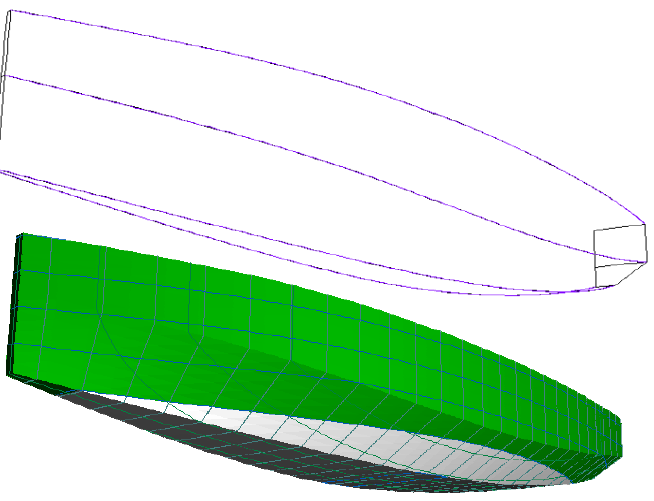
\includegraphics[width=0.5\textwidth,natwidth=654,natheight=501]{filecarene.png}
        \caption{}
        \label{fig:carene}
\end{wrapfigure}

\subsubsection{Import Carene XYZ file.}
This option is to open a textfile generated by the Carene program,
which is available from
\url{http://www.epoxy-resins.co.uk/Carene/carene.htm}. The textfile
contains the coordinates of the chines describing the hull. These
chines will be imported into ShipCAD and a spline is fitted such that
the chine in ShipCAD lies exactly on that of Carene. The original
chine as defined in the XYZ file is added as a marker so that it can
be checked visually if the models are the same. Controlcurves are
added to the crease edges corresponding to each chine.

\subsubsection{VRML.}
Import a mesh from VRML 1.0 files. For information regarding the VRML
format see:
\url{http://www.bergen.org/ATC/Course/InfoTech/VRML_FAQ.html}
\url{http://trap.mtview.ca.us/~tom/tech/languages/vrml10c.html}
When a VRML file is imported only the boundary-edges are set as crease-edges. All other crease-
edges must be manually set. The only information imported from a VRML file are indexed face sets.

\subsubsection{PolyCad files.}
Used to import .geo files generated with PolyCad by Marcus
Bole. PolyCad can be downloaded for free
from \url{http://www.polycad.co.uk/downloads.htm} Information
currently imported from the file includes either generalized Bspline
surfaces or surfaces generated with the Shiplines or Yachtlines
option. Contours are also imported.

\subsubsection{Michlet waves.} \label{michlet-waves}
If wave elevations have been calculated using Michlet
(see \ref{michlet} Michlet),
the results can be saved to a file. ShipCAD is able to import this
information back into the program. It is important not to use too many
panels. A resolution of 50 x 50=2500 panels gives generally a good
result as can be seen below. Using more panels really slows the
program down. Results of both the rectangular plot and the sectorial
plot can be imported into the program.

\begin{figure}[h]
        \centering
        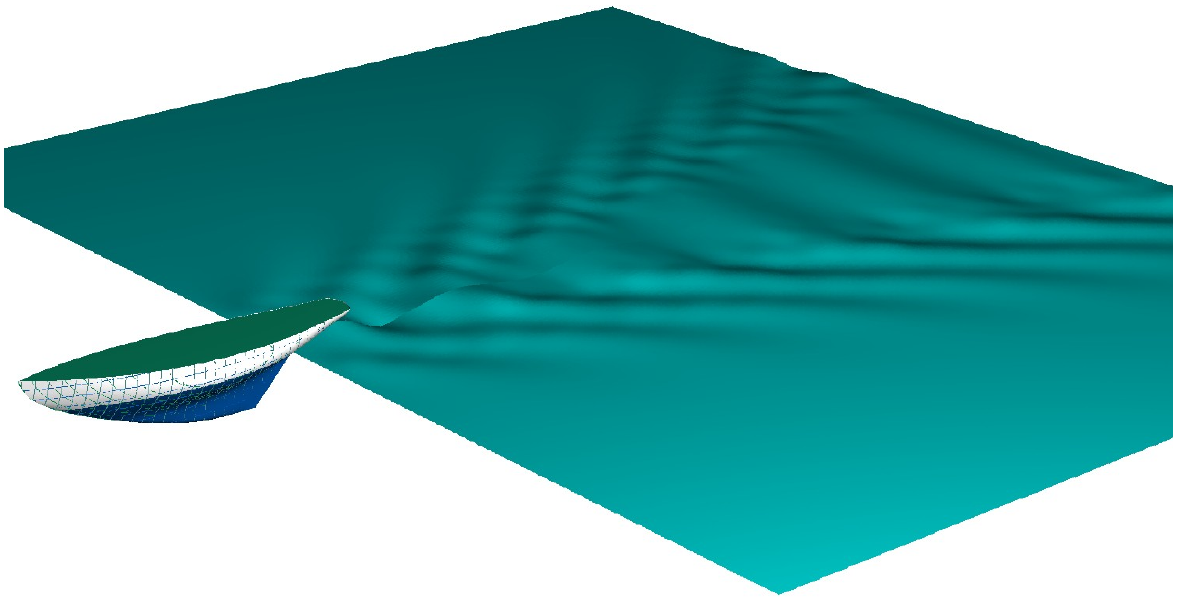
\includegraphics[width=15cm,natwidth=1182,natheight=601]{filemichlet.png}
        \caption{}
        \label{fig:filemichlet}
\end{figure}

\subsection{Export.}
ShipCAD currently exports the following file formats:

\subsubsection{Part.} \label{part}
It is possible to save a selection of the model as a part to a so
called part file. You can do this by selecting the desired faces
yourself, or by selecting layers in the layer selection dialog that
appears if no faces were selected manually. Apart from the points,
edges, faces and controlcurves also layer information is saved. This
way for example a keel can be saved to a file and imported in another
design.

\subsubsection{IGES.}
Subdivision surfaces can be used to model very complex shapes with
only one mathematical surface, which cannot be done with one single
NURB surface. Because of this it can be difficult to translate the
subdivision surface into NURB surfaces. Normally one NURB surface is
created for each face with 4 points. Faces with more or less points
are subdivided in as much NURB patches as there are points in the
face. So a three sided face is converted to 3 NURB patches. This can
lead to an enormous amount of patches in the IGES file. This is not
necessarily a problem, unless you want to modify the surfaces in
another CAD program. Therefore ShipCAD uses an algorithm that
assembles as much 4 sided faces as possible to form larger NURB
surfaces. This reduces the amount of exported surfaces
significantly. In some cases it can even be reduced to a single NURB
surface. Only surfaces are exported to the IGES file. They are
exported as NURB surfaces (IGES entity 128).

\subsubsection{DXF 3D mesh.}
The same algorithm as described above is used to form polygonal meshes. These meshes are
exported as DXF polymeshes. Faces that cannot be converted to meshes are exported as 3D
faces. 3D faces are small three or four sided surfaces used in AutoCad. The information send is
equal to what is visible in the viewport. Only visible layers are sent. If the viewport shows both
halves of the ship then both halves are exported.

\subsubsection{DXF 2D polylines.}
The intersection curves (except diagonals) can be exported to a 2D DXF file. A dialog appears in
which you can specify the directory where the files should be saved and the units in which they are
saved (meters, centimeters, millimeters, feet or inches). Each curve can be exported to a different
file, or curves can be grouped and saved to 3 files (stations, buttocks and waterlines). Because of
the fact that the curves are exported as polylines, curved sections are approximated by straight line
segments. The max. length of such a straight line segment is adjustable which makes this kind of
export ideal for CNC data.

\subsubsection{DXF 3D polylines.}
All intersection curves such as stations, buttocks, waterlines,
diagonals and crease edges are exported to an AutoCad DXF file as 3D
polylines. Controlcurves are exported also. Again information is
exported as visible in the viewports.

\subsubsection{Wavefront file (.obj).}
Visible parts of the surface are sent to an .obj file as specified at
\url{http://www.fileformat.info/format/wavefrontobj/}. Color information is not included at this point.

\subsubsection{STL file.}
The STL format is mainly used for manufacturing purposes, but
sometimes also for exchanging data with other CAD programs. All
visible parts of the surfaces are send to the file as a large
collection of small triangles.

\subsubsection{Export .fef file.}
See: \ref{import-fef}

\subsubsection{Offsets.}
Offsets of intersection curves and controlcurves are exported to a
text file. Regardless of the visibility settings all available lines
are exported. Of each line only the portside is send to the file.

\subsubsection{Coordinates.}
This option saves the coordinates of all the controlpoints from the
model to a textfile. This textfile can be read directly into Rhino.

\begin{wrapfigure}{r}{0.4\textwidth}
        \centering
        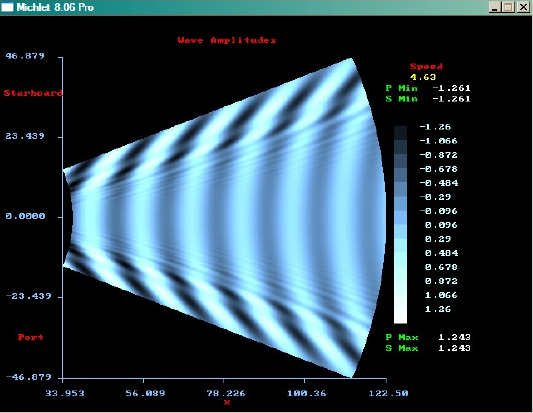
\includegraphics[width=0.4\textwidth,natwidth=533,natheight=413]{michletscreenshot.png}
        \caption{}
        \label{fig:michletscreenshot}
\end{wrapfigure}

\subsubsection{Michlet.} \label{michlet}
Michlet is an excellent free CFD program which can be downloaded from
\url{http://www.cyberiad.net/michlet.htm}. The program can be used to give a more accurate prediction
of frictional and residual resistance. It is based in Mitchell's
theory and is best suited for ships with a large length/beam ratio (7
or higher) and low blockcoefficient. However Leo Lazauskas, the author
of Michlet, reported that even ships with a L/B ratio of 5 and up may
be used, although this reduces accuracy. Michlet also predicts the
wave elevations of the far field (the waves behind the vessel). For
more information regarding the use of Michlet and its input values the
user is referred to to Michlet manual.  One important aspect which I
believe is not mentioned in that manual is that the speed used for
prediction wave elevations cannot be higher than the maximum speed
specified for the resistance calculations. So make sure that this is
high enough.  There are currently 3 ways of exporting a hull to
Michlet:

\begin{itemize}

  \item \textbf{Monohull}. This is the default option for sending monohulls.

  \item \textbf{Monohull as catamaran}. This option is intended for designing catamarans. The usual
way to do this is first design the hull as a monohull, with it's centerplane still on the XZ
plane through the origin. You can send the hull to Michlet as a multihull with a specified
distance between the two center planes of each individual hull. Michlet can be used to
optimize this distance by varying it as the interference of the two hulls shows up in the
wave pattern (and in the resistance curves).

  \item \textbf{Catamaran}. If you have a design consisting of two hulls, again the distance must be
specified. however in this case it \textbf{must} be the actual distance between the center planes
of the hulls otherwise ShipCAD cannot calculate the proper offsets of
the hulls.

\end{itemize}

If you want to use Michlet it is important to realize that each
individual hull in Michlet must be symmetrical with respect to its own
centerplane. In other words, it cannot handle asymmetrical hulls.  The
results of the wave elevation calculation can be imported back into
the program. More information about this topic is given in \ref{michlet-waves}.

\subsubsection{Archimedes.}
ShipCAD exports all stations in the model either to Archimedes single
body (.app file) or to ArchimedesMB, which is the multi body version
of Archimedes (.hll file). Both versions of Archimedes can be used to
perform additional hydrostatic and stability calculations. Archimedes
is low-cost software and is available
from \url{http://www.naval-architecture.co.uk}. This option is only
enabled if stations are added to the model.

\subsubsection{GHS.}
Export all available stations to a GHS file. GHS files can be imported
by most hydrostatic programs that perform calculations based on a
bodyplan and is a widely accepted format.

\subsection{Exit.}
Shuts down the program.

\subsection{Preferences.}
The following dialog in Illustration 11 shows in which program
preferences may be altered. These modified preferences are stored in
the file freeship.dta located in the same directory as the program. To
restore the preferences to the default settings it suffices to delete
this file and restart the program. You can restore modifications to
color settings by pressing the reset button.  You can also modify the
language used by ShipCAD. More about the language support can be found
in \ref{language-support}.

\begin{figure}[h]
        \centering
        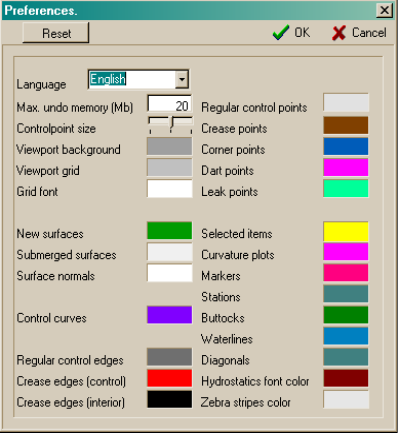
\includegraphics[width=10cm,natwidth=399,natheight=435]{preferencesdialog.png}
        \caption{}
        \label{fig:prefdialog}
\end{figure}

\pagebreak

\section{Project options.}

\begin{wrapfigure}{l}{0.4\textwidth}
        \centering
        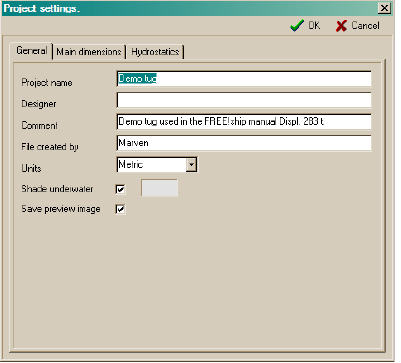
\includegraphics[width=0.4\textwidth,natwidth=401,natheight=363]{projectsettingsdialog-1.png}
        \caption{}
        \label{fig:projsettings1}
\end{wrapfigure}

\subsection{Project settings.} \label{project-settings}
The project settings dialog will let you specify various project
settings. It has a number of tab pages.

The first tab page is used for general information about the
project, such as the project name, name of the designer, some
comment, the name of the person who created the file and the
type of units used for this project. This can either be imperial or
metric units.

It is also possible to turn shading of the submerged hull in a
different color on or off, and to specify the color to be used for the
submerged body.

There's also a switch to enable or disable the storage of a
preview image in the project file.

\begin{wrapfigure}{l}{0.4\textwidth}
        \centering
        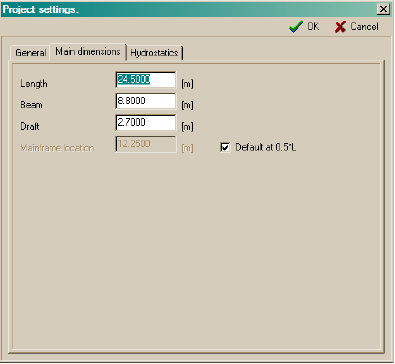
\includegraphics[width=0.4\textwidth,natwidth=395,natheight=364]{projectsettingsdialog-2.png}
        \caption{}
        \label{fig:projsettings2}
\end{wrapfigure}

The second tab page is used to define the main particulars of the
model, and the location of the midship section. By default this is
at half the defined project length but this can be modified.

\begin{wrapfigure}{l}{0.4\textwidth}
        \centering
        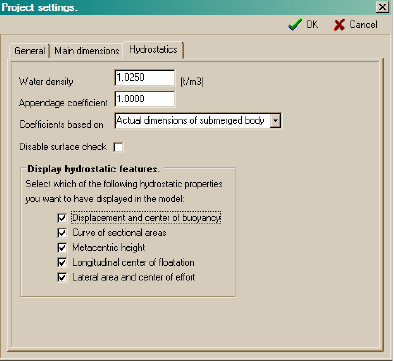
\includegraphics[width=0.4\textwidth,natwidth=394,natheight=361]{projectsettingsdialog-3.png}
        \caption{}
        \label{fig:projsettings3}
\end{wrapfigure}

The last tab page is used for all hydrostatics related settings, such
as the density of the water and appendage coefficient. This is a
factor normally used to incorporate shell thickness and appendages
such as the rudder in the displacement calculation, usually in the
range 1.005 - 1.010. There's also a dropdownbox which can be used to
specify how hydrostatic coefficients, such as for example the
blockcoefficient and prismatic coefficient should be calculated. This
can be done using either the dimensions specified in this project
dialog (customary when designing larger ships) or the actual
dimensions of the submerged body(customary when designing yachts and
small boats).

Each time hydrostatics are calculated, the program checks the
direction of all facenormals. If the normals point in the wrong
direction after this check, it is best to disable the automatic check
and manually flip the normals (\ref{flip}) to the correct side.  ShipCAD
can also show some hydrostatic features in the 3D model in wireframe
mode (see \ref{hydrostatic-features}). You can also specify here which
features should or should not be plotted.

\subsection{Linesplan.}
ShipCAD enables the user to view the complete formatted linesplan of
the ship. This can be done in two different modes, wireframe mode (to
the left) and the filled mode (to the right). The linesplan shows only
the present intersection curves, regardless of the visibility setting
of the corresponding intersection curves. So stations are always shown
in the linesplan, even if they are switched off in the hullform
views. Currently this linesplan can be saved as a bitmap, to a dxf
file, or sent directly to the printer/plotter. The linesplan can also
be drawn in black \& white by clicking on the appropriate button in
the toolbar. Using fill colors is not possible in black \& white
mode. Only if the model contains \underline{no} diagonals, the plan view might
optionally be mirrored so that both sides are visible.

\begin{wrapfigure}{r}{0.7\textwidth}
        \centering
        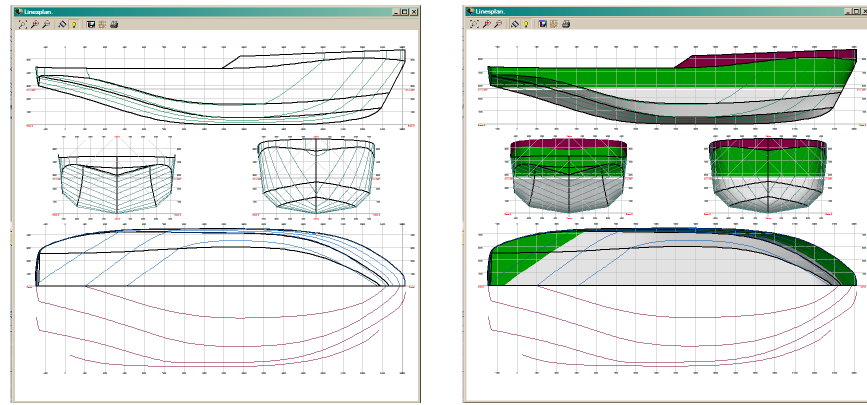
\includegraphics[width=0.7\textwidth,natwidth=867,natheight=405]{linesplan.png}
        \caption{}
        \label{fig:linesplan}
\end{wrapfigure}

Some layers can be hidden from the linesplan. How this is done is
described in
\ref{layer-properties}.

\pagebreak

\section{Edit menu.}

\subsection{Undo.}
Undo previous editing actions. ShipCAD stores all actions. When a new
file is read into memory, the previous undo data will not be
destroyed.

\subsection{Delete.}
Use this if you want to delete selected items. The program first
deletes all selected faces, then the edges and finally the selected
points. Any points or edges that appear to be unused after this
process are deleted also. Note that when a point is deleted all
attached faces and edges are deleted too. If an edge is deleted, any
attached faces will also be deleted. See also \ref{point-collapse}
and \ref{edge-collapse}.

\pagebreak

\section{Point operations.}

\subsection{Add.}
Adds a new point in 3D space. The new point is by default located at
the origin (0.0, 0.0, 0.0).  Adding new points is only enabled if the
controlnet is visible.

\subsection{Align.}
If more than two points are selected it is possible to align them so
that they form a straight line. This is done by projecting all the
selected points on the line segment through the first and last
selected point. They are projected to that line rather than uniformly
distributed to keep the displacement of the points minimal.

\subsection{Collapse.} \label{point-collapse}
This removes a selected point without deleting the surrounding
geometry. A point can only be collapsed if it is attached to exactly
two edges. The point is then removed, and the two edges are combined
into a single edge. If a point is attached to more than 2 edges, the
other edges might be removed first by collapsing these edges. The
example below shows a point before and after collapsing it.

\begin{figure}[h]
        \centering
        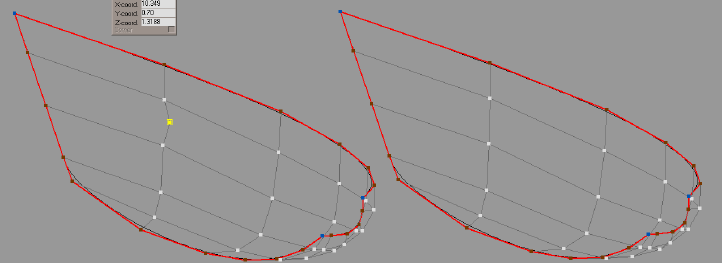
\includegraphics[width=12cm,natwidth=723,natheight=264]{pointcollapse.png}
        \caption{}
        \label{fig:pointcollapse}
\end{figure}

\subsection{Insert.}
For inserting a new point on an existing edge the reader is referred
to the edge-split operation.

\subsection{Insert plane.}
This operation intersects all edges that are \textbf{visible} with a
plane. If such an intersection point exists, it will be inserted on
the edge. After this, faces that have multiple newly inserted points
will be split by inserting a new edge. This is a convenient way to
insert for example a while range of points at a certain ordinate
location. There is also an option to add a controlcurve to the newly
created edges.  The type of plane (vertical, horizontal or transverse)
can be specified as well as the location by entering the desired
distance into the dialog that appears.

\subsection{Intersect layers.}
This option is used for finding the intersection curve of two layers,
so it is only enabled if more than one layer exists. If two layers are
selected than all the edges of the first layer are check for an
intersection with all the faces of the second layer. If such an
intersection exists than the point is inserted in the edge. After the
intersection test all inserted points are connected with new edges
which form the intersection curve of the two layers. Remember that
only the first layer is affected by this operation, the second layer
is left undisturbed. Another important issue is that points are only
inserted in edges, \textbf{not} in faces. This option can be used for example
to find the intersection of the hull with a keel or rudder.

\subsection{Lock points.}
All selected unlocked points will be locked. Locked points appear dark
gray on screen and cannot be moved. None of the available editing
operations has any effect on locked points. This option is only
enabled when more than 1 unlocked point is selected.

\subsection{Unlock points.}
This unlocks selected points that are locked, so that they can be
modified again. Only enabled if at least 1 of the currently selected
points has previously been locked.

\subsection{Unlock all points.}
This unlocks all points in the model, whether they are selected or not.

\pagebreak

\section{Edge operations.}

\begin{wrapfigure}{r}{0.4\textwidth}
        \centering
        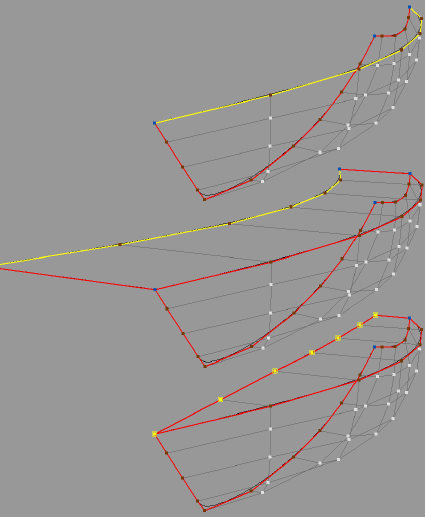
\includegraphics[width=0.4\textwidth,natwidth=426,natheight=517]{edgeextrude.png}
        \caption{}
        \label{fig:edgeextrude}
\end{wrapfigure}

\subsection{Extrude.}
Extruding edges is a convenient way to create new surfaces.  Since an
edge may only have a maximum of two faces attached, only
boundary-edges are allowed to be extruded.
Figure \ref{fig:edgeextrude} shows how a deck is easily added by
extruding the sheerline. The three stages of the process are:

\begin{itemize}

\item Select the boundary edges that must be extruded.
Select the edge-extrude option from the menu. A
dialog appears in which the direction of the extrusion is
specified. In this case the extrusion direction is 0.0 in
longitudinal direction, -2.25 in transverse direction and
0.02 upwards.

\item The edges are extruded in the specified direction. New
faces are created and added to the currently activelayer. (See \ref{general-info-layer}
General information about layers)


\item The newly created points are moved to the centerline, and the deck is finished.

\end{itemize}

\begin{wrapfigure}{r}{0.4\textwidth}
        \centering
        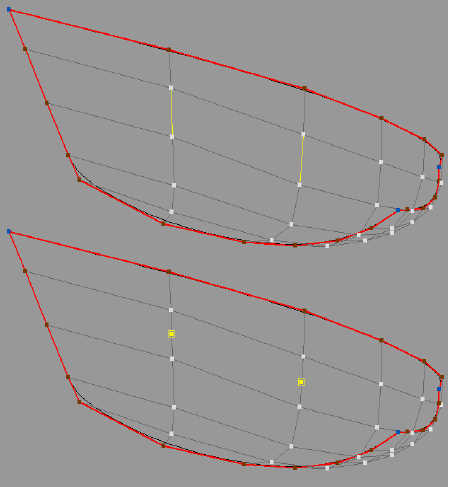
\includegraphics[width=0.4\textwidth,natwidth=449,natheight=487]{edgesplit.png}
        \caption{}
        \label{fig:edgesplit}
\end{wrapfigure}

\subsection{Split.}
Selected edges are split in two by inserting a new
point in the middle. After the operation all newly
created points are selected. This is convenient if new
edges should be inserted. In that case multiple edges
can be selected and split in two. All selected points
belonging to the same face may then be split by
inserting a new edge. (see \ref{edge-insert} Insert). The image to
the right shows two selected edges before and after
the split. Note that this way a face consisting of 6
points is created. The two selected points should
preferably be connected, thus splitting the face in two
regular faces. This ensures a more regular grid and a
smoother surface. (see also \ref{guidelines} Guidelines to
subdivision modeling).

\subsection{Collapse.} \label{edge-collapse}
Collapsing an edge removes the edge and combines the two attached
faces into one new face.  Edge collapsing only makes sense if the
selected edge is not a boundary-edge. The example to the right shows
how multiple edges are collapsed in one pass. Only two points on the
boundary-edges remain. These can be collapsed using the point-collapse
option from the menu.

\begin{wrapfigure}{r}{0.3\textwidth}
        \centering
        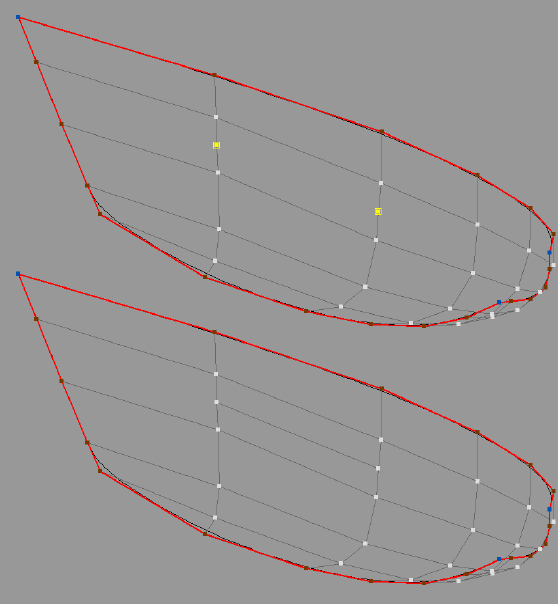
\includegraphics[width=0.3\textwidth,natwidth=560,natheight=605]{insertedge.png}
        \caption{}
        \label{fig:edgeinsert}
\end{wrapfigure}

\subsection{Insert.} \label{edge-insert}
A face can be split into two new faces by inserting an edge. To do
this at least two points have to be selected. Both points must share
the same face, and no edge is allowed to already exist between these
two points. To ensure a fair surface it is recommended to extend
inserted edges (as those seen to the right) to a crease or
boundary-edge if possible.

\begin{figure}[h]
        \centering
        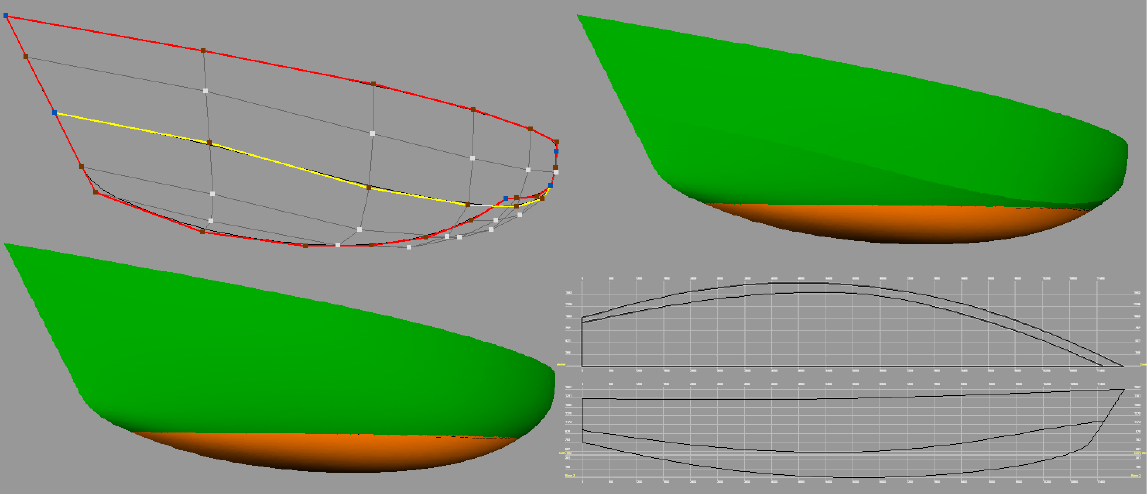
\includegraphics[width=15cm,natwidth=1147,natheight=495]{creaseedge.png}
        \caption{}
        \label{fig:creaseedge}
\end{figure}

\subsection{Crease.}
Setting selected edges as crease-edges allows the user to add knuckle
lines to the hull. The crease-property of boundary-edges cannot be
changed. ShipCAD treats all boundary edges by default as
crease-edges. The image below shows how a hard chine is created. To
the left the model without the chine is visible. To the right the
yacht with the new knuckle line is displayed. In this specific example
the knuckle line runs over the full length of the hull. This is not
absolutely necessary. Knuckle lines may run freely over the surface.
Illustration 17

\pagebreak

\section{Curve operations.}

\subsection{Controlcurves and fairing.}
To have a better control over the shape of the surface, controlcurves
can be added to the model.  These controlcurves are assigned to edges,
and after each subdivision step the new edge-points are not only
inserted into the surface but also into the curve. This ensures that
the controlcurves are always exactly embedded in the surface,
regardless of the precision setting of ShipCAD. If the curvature
visibility is switched on, then the curvature plot of the selected
controlcurves is shown also. This curvature plot is updated in
realtime if one of the points is moved. If the curvature plot is
interpreted and used correctly it is possible to produce a perfectly
fair surface. Bumps or dents in the surface that are too small to be
seen on screen with the naked eye are easily identified.  So what is
curvature anyway? Curvature can be defined as follows:

\begin{center}
\textit{the rate of change (at a point) of the angle between a curve and a tangent to the curve}
\end{center}

\begin{figure}[h]
        \centering
        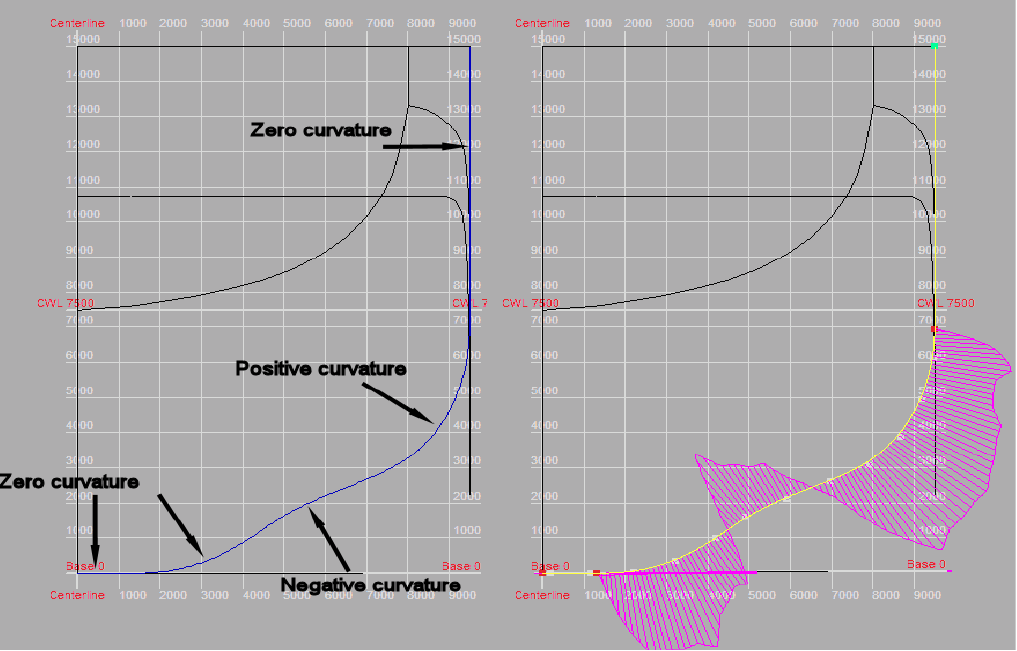
\includegraphics[width=15cm,natwidth=1017,natheight=651]{curvature.png}
        \caption{}
        \label{fig:curvature}
\end{figure}

The image above shows a controlcurve in the aft part of a container
ship. To the left the controlcurve is shown in blue, while to the
right the controlcurve is show in a selected state (yellow) together
with it's curvature plot (fuchsia). The straight parts of the curve
have zero curvature. If you travel along the curve from the bottom to
the direction of the deck, first the curve starts bending to the
left. In this area the curvature is positive. At a height of about 2.5
meters the curve starts bending to the right, here the curvature
becomes negative. A little bit further along the curve it bends to the
left again, so the curvature becomes positive. How is this translated
into the curvature plot? At a number of points on the curve the
curvature is calculated and drawn as a line, perpendicular to the
curve. The larger the line, the larger the curvature. If the curvature
is positive the line is drawn on the opposite site of the curve. So
while the absolute value of the curvature in a point is not that
interesting, the way it changes along the curve is. This is a measure
of the fairness of the curve. You don't want abrupt changes in the
curvature, it should vary as smoothly as possible. And very often,
especially with small boats and yachts, a change of the sign of the
curvature as seen in the image above is highly undesirable. Below is
an example of a controlcurve from a sailing yacht. The upper part of
the image shows a poorly faired curve. We see a change of the
curvature sign in an area where it should be positive, followed
shortly after that by a sudden increase in the size of the
curvature. After that the curvature size rapidly drops, just to
increase again at the bow. The lower half of the image shows the same
controlcurve after being faired. It is obvious that the curvature
changes gradually now and the curve is very smooth.

\begin{figure}[h]
        \centering
        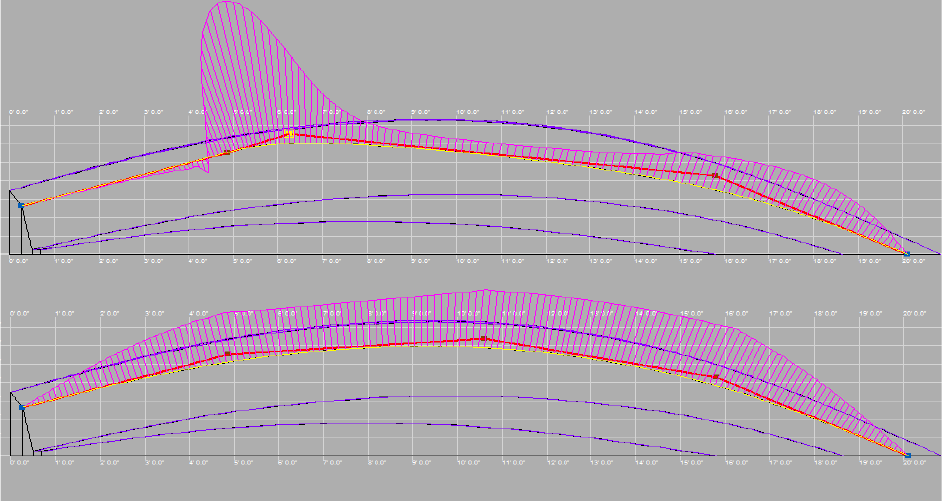
\includegraphics[width=15cm,natwidth=943,natheight=503]{linefairing.png}
        \caption{}
        \label{fig:linefairing}
\end{figure}

One thing to bear in mind is that the curvature at the first and the
last point of the curve is always zero. This is due to the way the
curve is being drawn, and it has nothing to do with the actual
curvature of the surface at that point. Controlcurves are easier to
fair when the controlpoints are spaced more or less evenly along the
curve and are regular whenever possible. The less controlpoints a
curve has, the easier it is to produce a good running smooth curve.

\subsection{New}
First select a number of edges that are connected by their start and
endpoints. (This is easier when you hold the control key on your
keyboard pressed down when selecting an edge) After that it is
possible to create and assign a controlcurve to these edges. Only one
controlcurve can be assigned to each edge. If the new curve is not
shown on the screen, make sure that the visibility of controlcurves is
turned on.

\pagebreak

\section{Face operations.}

\subsection{New.}
Add a new face using previously selected points. These points have to
be selected in the correct order. If looked in the direction of the
new face as seen from the water, the normal of the new face points
outward if the points are sorted in counterclockwise order. If
selected in clockwise order, the normal points inward. All
normals \textbf{must} point outward in the direction of the water (see
1.6 Guidelines to subdivision modeling). The direction of facenormals
is automatically checked and corrected (if possible) if this option is
not disabled in the project dialog. This check is performed each time
hydrostatics are calculated or when the check model option is chosen
from the menu.

\subsection{Flip.} \label{flip}
This option can be used to manually flip the normals of selected faces
to the other side. The normals of a face can be visualized by
selecting the specific face. Make sure that both interior edges and
visibility of normals are turned on. When displaying normals, each
normal is calculated as the average normal in a point of the refined
subdivision mesh. This average is calculated from all faces
surrounding that point. Along the boundary of an edge sharing two
faces with opposite normal directions, this may seem a bit strange as
can be seen on the left side of the image below. The normals along
these boundaries look as if projected to the surface.

\begin{figure}[h]
        \centering
        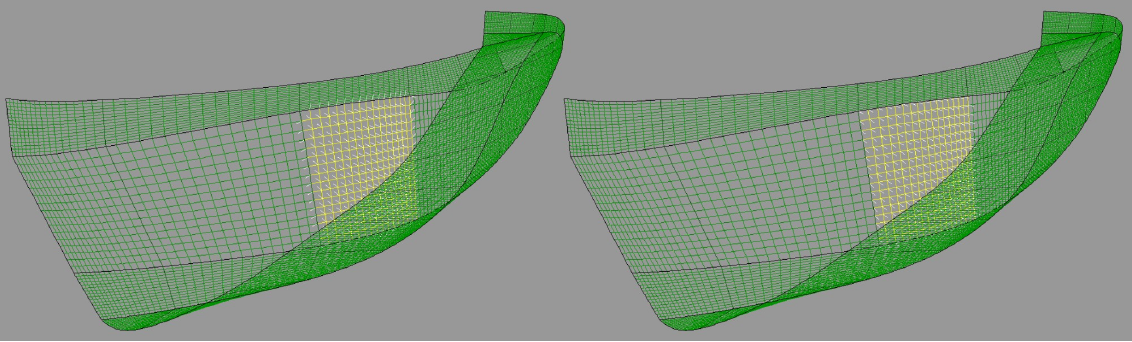
\includegraphics[width=15cm,natwidth=1132,natheight=342]{flipnormal.png}
        \caption{}
        \label{fig:flipnormal}
\end{figure}

\pagebreak

\section{Layer operations.}

\subsection{General information about layers.} \label{general-info-layer}
The hull created with ShipCAD consists of only 1 surface, even if
multiple separate surfaces appear on the screen that are not connected
to each other. When modeling complex models the information on the
screen may sometimes be overwhelming. Therefore layers are
implemented.  Each face is assigned to a layer. These layers have
certain properties such as for example color and visibility. This way
it is possible to group faces into a layer and assign those properties
to all faces. The visibility property of these layers makes it
possible to hide them from the user. If all faces attached to an edge
or point are invisible, the edge or point in question will also not be
shown. This ensures an optimal view on the model when selecting items
or dragging points. Faces assigned to a layer all share the properties
of that layer.

\begin{wrapfigure}{r}{0.3\textwidth}
        \centering
        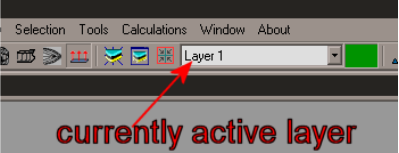
\includegraphics[width=0.3\textwidth,natwidth=399,natheight=153]{activelayer.png}
        \caption{}
        \label{fig:activelayer}
\end{wrapfigure}

\subsection{Active layer.}
At all times an active layer is present in the
model. If \textbf{\underline{no} faces are selected}, the dropdown box
in the toolbar displays which layer is currently active. If one or
more faces are selected belonging to the
\textbf{same} layer, this dropdown box shows which layer this is. This might be
a different layer then the active layer. When multiple faces are
selected which are assigned to \textbf{different layers}, the dropdown
box turns blank. All newly created faces created by extruding edges or
manually adding faces, are assigned to the layer which is currently
active.

\begin{wrapfigure}{r}{0.3\textwidth}
        \centering
        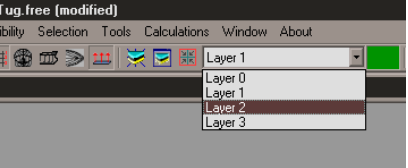
\includegraphics[width=0.3\textwidth,natwidth=408,natheight=168]{assignlayer.png}
        \caption{}
        \label{fig:assignlayer}
\end{wrapfigure}

\subsection{Assigning faces to a different layer.}
Assigning faces to a different layer is done as follows:

\begin{itemize}

  \item Select the faces in question
  \item Pull down the dropdown box and click on the new
layer.

  \item Deselect the faces.

\end{itemize}

All faces should now be assigned to the new layer.

\subsection{Active layer color.}
Modify the color of the active layer. This color is also visible in
the toolbar, right next to the dropdown box.

\subsection{Auto group.}
This option extracts groups of faces which are totally surrounded by
crease edges. Then each group of faces is assigned to a new layer. If
no faces are selected, all faces of the model will be used. Otherwise
only the selected faces will be grouped. ShipCAD tries to save as much
of the present information as possible. If a set of faces is
extracted, and they already belong to the same layer then this layer
is left undisturbed. Auto grouping is only enabled when interior edges
are turned on.

\begin{wrapfigure}{r}{0.3\textwidth}
        \centering
        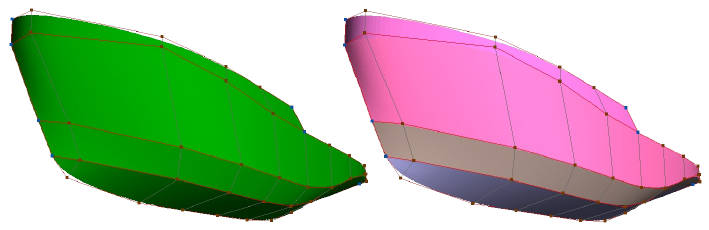
\includegraphics[width=0.3\textwidth,natwidth=709,natheight=230]{newlayer.png}
        \caption{}
        \label{fig:newlayer}
\end{wrapfigure}

\subsection{New.}
Adds a new empty layer to the model and makes it the active layer.

\subsection{Delete empty.}
Only enabled when the model contains at least one empty layer and when
more than 1 layer is present. When selected, all empty layers are
removed from the model. This also includes the active layer if it is
empty. At least one layer remains as the active layer.

\begin{wrapfigure}{r}{0.4\textwidth}
        \centering
        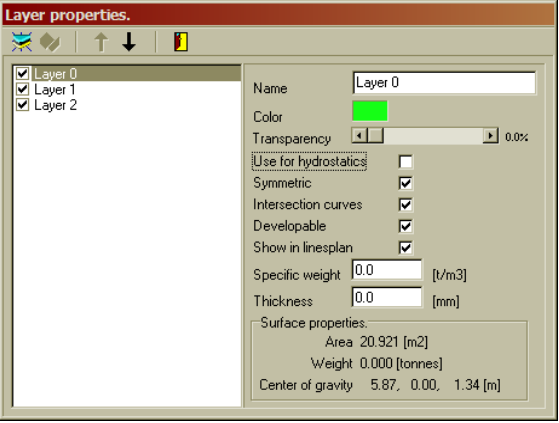
\includegraphics[width=0.4\textwidth,natwidth=559,natheight=423]{layerproperties.png}
        \caption{}
        \label{fig:layerproperties}
\end{wrapfigure}

\subsection{Layer properties dialog.} \label{layer-properties}
A window is displayed showing all layers and their properties. The
left half of the window shows a list containing all available layers
in the model.  By clicking on the name of a layer, this layer is
selected. The properties of this selected layer are then displayed to
the right. Double clicking on a layer in the list on the left side
makes it the active layer. From within this dialog it is possible to
turn layers on or off or to modify the following layer properties:

\begin{wrapfigure}{r}{0.3\textwidth}
        \centering
        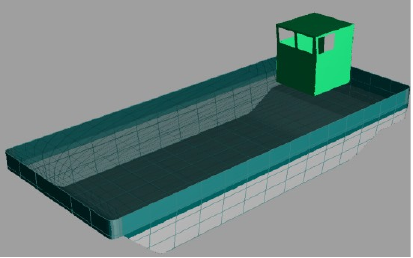
\includegraphics[width=0.3\textwidth,natwidth=413,natheight=258]{layertransparent.png}
        \caption{}
        \label{fig:layertransparent}
\end{wrapfigure}

\begin{wrapfigure}{r}{0.5\textwidth}
        \centering
        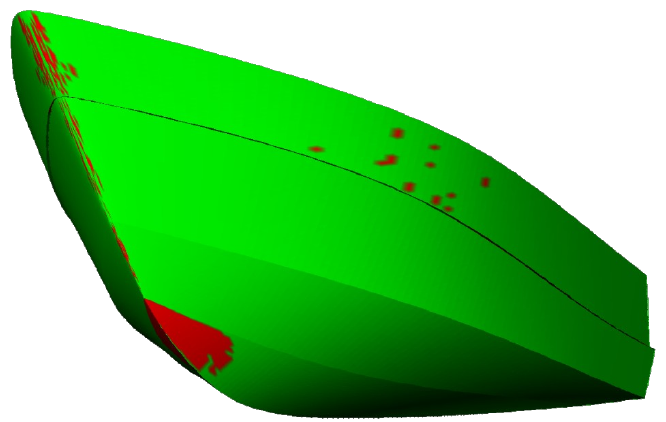
\includegraphics[width=0.5\textwidth,natwidth=666,natheight=422]{developable.png}
        \caption{}
        \label{fig:developable}
\end{wrapfigure}

\begin{itemize}

\item Visibility.
The checkboxes on the left side indicate whether the corresponding
layer is visible or not. Click on the checkbox to turn the layer on or
off. Points or edges from the controlnet belonging to invisible layers
are also hidden, which makes modeling of complex models easier.

\item Name.
The layer name is displayed in the list at the left, but it can only
be modified at the right side of the window. ShipCAD does not require
the layer name to be a unique name, since all layers are identified by
an internal unique identification number. Some CAD programs however,
such as Autocad, do not allow spaces in the name of a layer or
duplicate names.

\item Color.
The layer color is used for shading the model. It is also used in the
linesplan and for developed panels. The color of a layer can be
modified by clicking the colored square to the right. A dialog then
appears in which a new color can be chosen.

\item Transparency.
Sometimes it is nice to shade certain surfaces (partially)
transparent, such as windows for example. The amount of transparency
can be modified by moving the slidebar.  The amount of transparency
can range from 0% (totally solid) to 100% (invisible). Note though
that transparent shading might consume a lot of memory and
significantly slow down the shading process. Since normal Z-buffer
shading or plain alpha blending produces strange artifacts, the only
way to do this properly is by keeping track of all surfaces covering a
particular pixel on the screen and then drawing all these surfaces
from the back to the front. This costs extra memory and CPU time, but
apart from being a bit slower it should not pose any real problems.

\item Symmetric.
Only if a layer does \textbf{not} contribute the hydrostatics it can be a
non-symmetrical layer. So generally it can not be used to create
asymmetrical hulls. It can be used however to add asymmetrical
deckhouses or other objects on the hull, such as sails, people etc.

\item Use for hydrostatics.
ShipCAD uses the faces of the subdivision mesh for hydrostatic
calculations (see \ref{design-hydrostatics} Design hydrostatics). It
calculates the volume enclosed by these faces. Sometime however there
are surfaces present in the model that should not be included in the
hydrostatic calculations. This is particularly the case if the faces
of a layer do \textbf{not} form an enclosed volume, but only a
surface, such as a sail for example. If a sail were to be included in
the calculations, ShipCAD would calculate the volume aft of the sail
(if it is submerged) as a volume. Since this volume extends to
infinity (there is no backside surface present) it would introduce an
error. So specific layers can be excluded from the calculations by
removing the check from the checkbox. See also \ref{check-model} Check
model for more information concerning leak points.

\item Intersection curves.
By clicking this checkbox, the intersection curves property of a layer
can be enabled or disabled. If the checkbox is not checked then the
faces of this layer will not be included when the intersection curves
are calculated. For complex models it is often convenient to display
stations, buttocks, waterlines and diagonals of the hull only, and not
for the deck, superstructure etc. This setting has \textbf{no} influence on the
hydrostatics.

\item Developable.
Developable hulls can be build from flat plates which are only bend in
one direction. Most hulls are not developable since the surface is
curved in two directions.  Layers from which the developable property
is checked are shaded differently. Developable areas of these layers
are shaded with a light green color. Areas that are not developable
are shaded red. This is a convenient way to check if a hull is indeed
developable.  Illustration 22 shows an example of a multi-chine
motorboat. It can immediately be seen by the green Illustration 22
color that almost the entire hull is developable. Just a few very
small spots in the topside and bow, and a larger area in front at the
bottom are colored red. Those very small spots are mostly numeric
errors (ShipCAD uses a very small tolerance). The larger bottom area
however is not developable from a mathematical point of
view. Developable hulls are often made of plywood, which is far easier
to bend than metal as a result of different material properties. In
reality “almost” developable hulls can perfectly be build using
plywood, whereas the same hull build of metal requires “torturing” the
metal to get it into shape. If one or more layers are marked as
developable, the program can unfold (or develop) this 3D surface onto
a flat plane as explained in \ref{develop-plates} Develop plates.

\item Show in linesplan.
Sometimes a layer contains items you don't want to be seen in the
linesplan. An example of this could be a mast and sails. These are
relatively high compared to the rest of the boat.  Showing these in
the linesplan view would cause the hull to appear very
small. Therefore some layers may be hidden. Be aware though that the
scale of items in the linesplan is also determined by the intersection
curves. If a layer would contain a sail, and the intersection curves
property is checked, intersection curves of this sail would still be
calculated and seen in the linesplan. Therefore it is best if you want
to hide layers from this view to also disable calculating intersection
curves from those layers.

\item Material properties.
There are two input fields at the bottom that can be used for a weight
estimation of a layer. In the “specific weight” field the density of
the used material can be entered, for example 7.8 tons/m3 in the case
of steel. In the field below that the average thickness can be
specified. These two properties combined with the total area of the
surface assigned to this layer result in a weight estimate and
corresponding center of gravity. This is shown when the design
hydrostatics are calculated.

\end{itemize}

Below the material properties the surface area, weight and center of
gravity of the selected layer are displayed. The black up and down
arrows in the toolbar can be used to move a selected layer up or down
in the list. Developable layers will appear in the same order in the
window with developed panels.

\pagebreak

\section{Visibility options.} \label{visibility-options}

\begin{wrapfigure}{r}{0.4\textwidth}
        \centering
        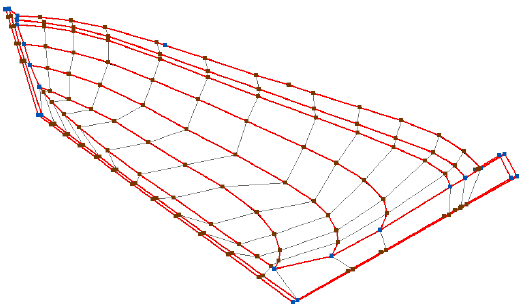
\includegraphics[width=0.4\textwidth,natwidth=529,natheight=308]{controlnet.png}
        \caption{}
        \label{fig:controlnet}
\end{wrapfigure}

\subsection{Control net.} \label{control-net}
The controlnet is the combination of points and edges that form the
initial subdivision mesh.  These are the entities that can be
manipulated by the user to shape the surface. If all the faces
attached to a certain point or edge belong to layers which are turned
off, it will not be drawn to the viewports. That way only the points
or edges of interest will be shown.

\subsection{Controlcurves.}
Controlcurves are curves that are assigned to edges of the controlnet
and are used to fair the surface. The visibility of these control
curves is not depending on the visibility of the controlnet.  In fact,
selecting and manipulating controlcurves is often easier when the
control net is not visible. Points and edges assigned to a
controlcurve automatically become visible whenever a controlcurve is
selected.

\begin{wrapfigure}{r}{0.4\textwidth}
        \centering
        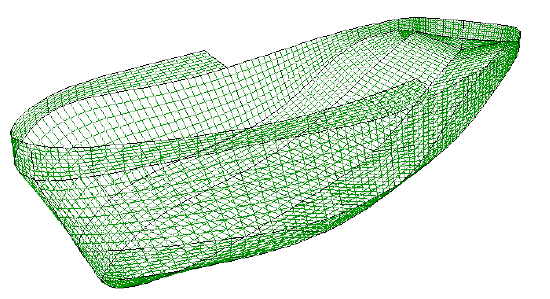
\includegraphics[width=0.4\textwidth,natwidth=559,natheight=299]{interioredges.png}
        \caption{}
        \label{fig:interioredges}
\end{wrapfigure}

\subsection{Interior edges.} \label{interior-edges}
The interior edges are in fact the edges of the subdivided
surface. The higher the precision is set, the more edges are
shown. The interior edges are drawn in the color of the layer they are
assigned to.

\begin{wrapfigure}{r}{0.4\textwidth}
        \centering
        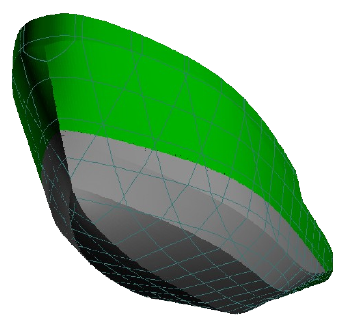
\includegraphics[width=0.4\textwidth,natwidth=350,natheight=317]{showbothsides.png}
        \caption{}
        \label{fig:showbothsides}
\end{wrapfigure}

\subsection{Show both sides.}
Since almost any ship is symmetrical in respect to the centerplane,
only the portside of the hull is modeled. If less information is shown
it is easier to select a point, edge or face. Both sides can be shown
however so that the designer has a good impression of what the entire
hull looks like.  Not only the surface is drawn symmetrical, also the
intersection curves. Showing both sides of the hull is possible in
both wireframe view and shaded view.

\begin{figure}[h]
        \centering
        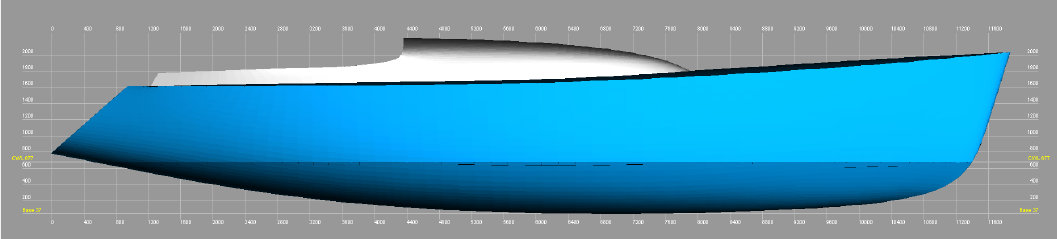
\includegraphics[width=15cm,natwidth=1057,natheight=239]{grid.png}
        \caption{}
        \label{fig:grid}
\end{figure}

\subsection{Grid.}
If intersection curves are added it is also possible to have a grid
displayed. This grid marks the location of these intersection
curves. It is visible in wireframe and shaded mode and next to each
line its distance is printed. In addition the baseline, centerline and
dwl are also indicated. The grid is visible in all views except for
the perspective view. This grid is shown, regardless of the visibility
setting of the intersection curves.

\subsection{Stations.}
Draws all present stations to the viewport. This option is only
enabled if stations are added to the model.

\subsection{Buttocks.}
Draws all present buttocks to the viewport. This option is only
enabled if buttocks are added to the model.

\subsection{Waterlines.}
Draws all present waterlines to the viewport. This option is only
enabled if waterlines are added to the model.

\subsection{Diagonals.}
Draws all present diagonals to the viewport. This option is only
enabled if diagonals are added to the model.

\subsection{Hydrostatic features.} \label{hydrostatic-features}
FREEship also provides the option to plot some key hydrostatic values
in the model. These are:

\begin{wrapfigure}{r}{0.4\textwidth}
        \centering
        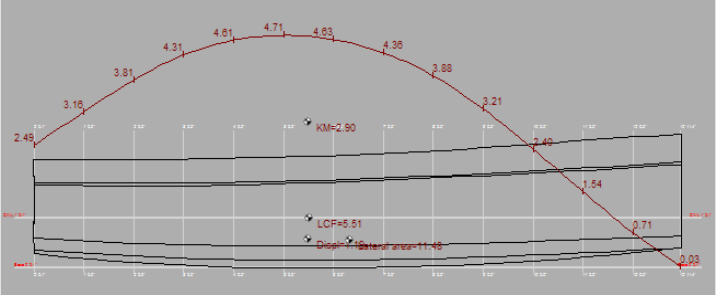
\includegraphics[width=0.4\textwidth,natwidth=717,natheight=296]{hydrostaticfeatures.png}
        \caption{}
        \label{fig:hydrostaticfeatures}
\end{wrapfigure}

\begin{itemize}

\item Center of buoyancy

\item Displacement

\item Center of floatation

\item Lateral center and area

\item Metacentric height

\item Curve of sectional areas. Contrary to the other values this
curve is \underline{only} plotted in the profile view
of the hull. Of course these values can only be shown if the model is
consistent enough to calculate the hydrostatics at the design draft
(so no leaks below the waterline). The values are updated in realtime
when the model is being modified. You can specify which data you want
the program to show in the project settings dialog (see \ref{project-settings} Project
settings).

\end{itemize}

\begin{wrapfigure}{r}{0.4\textwidth}
        \centering
        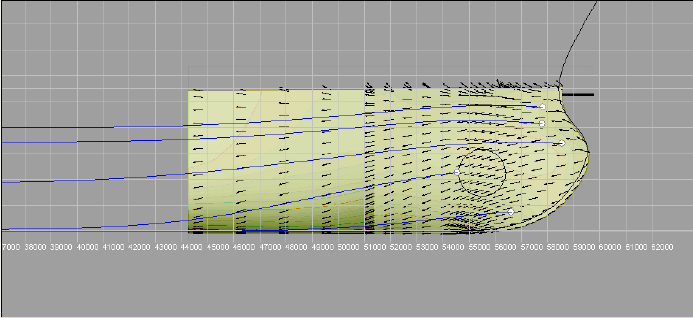
\includegraphics[width=0.4\textwidth,natwidth=693,natheight=318]{flowlines.png}
        \caption{}
        \label{fig:flowlines}
\end{wrapfigure}

\subsection{Flowlines.}
Show or hide flowlines. The flowlines that are displayed by ShipCAD
are calculated through analysis of the surface geometry only and have
nothing to do with CFD. This is a huge simplification as speed,
pressure and waves are excluded from the calculation. Despite this
simplification the flowlines show a resemblance with those calculated
wit CFD programs, but they only are added to give the designer an
impression of how the water will approximately flow. Real CFD
calculations are of course much more accurate and reliable. You can
add a flowline by keeping the alt-button pressed and clicking with the
mouse on a point below the waterline surface (profile, plan or
bodyplan view only). This point is used as the origin of the
flowline. From there the flow is traced as far as possible to the
stern or until it penetrates the design waterline. Flowlines are only
traced along surfaces that belong to a layer that is also used for
hydrostatic calculations (generally the shell of the hull). The image
above shows some flowlines at the bow of a hull with a bulb. The
background image shows the results from a CFD calculation. The small
black lines represent the direction of the flow as calculated with
CFD, the blue curves are the flowlines calculated by
ShipCAD. Flowlines can be selected and deleted like any other geometry
in ShipCAD.

\begin{wrapfigure}{r}{0.3\textwidth}
        \centering
        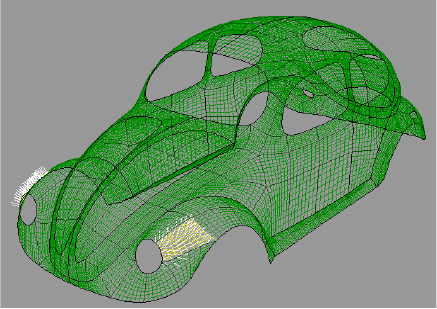
\includegraphics[width=0.3\textwidth,natwidth=437,natheight=309]{normals.png}
        \caption{}
        \label{fig:normals}
\end{wrapfigure}

\subsection{Normals.}
If this option is switched on, normals of \textbf{selected} faces are
drawn. The normals appear as thin white lines, pointing either inward
or outward the hull. This option is only enabled if the interior edges
are visible. A normal is drawn at each interior point of the
subdivision surface. The higher the precision is set, the more normals
are drawn.

\subsection{Curvature.}
This option enables or disables the drawing of the curvature plot of
certain intersection curves. Only of intersection curves which appear
checked in the intersection dialog will the curvature be plotted.

\subsection{Markers.} \label{vis-markers}
Markers are lines and/or curves added to the model as a reference. For
example the bodyplan of an existing design could be imported as
markers. Stations could then be added to the ShipCAD model at the same
location as the markers. Finally the points can be dragged until the
stations and the markers are exactly on top of each other. In that
case the ShipCAD hull matches the hull from the existing design.

Markers can be selected with the mouse and deleted like any other
geometry used in your model.

\subsection{Curvature scale.}
The curvature scale can be decreased by pressing the F9 key, so that
curves with high curvature can be evaluated. The scale can be
increased with the F10 key for low curvature areas.

\pagebreak

\section{Selection.}

\subsection{Select all.}
With this command (also available by pressing the shortcut Ctrl-A) all visible geometry can be
selected in one pass. This includes markers and flowlines.

\subsection{Deselect all}
Use this option to deselect all currently selected items simultaneously. Pressing the Esc-key has
the same result.

\pagebreak

\section{Tools.}

\subsection{Check model.} \label{check-model}
ShipCAD can check the model for any inconsistencies, and corrects most
of them automatically.  This check is also performed each time
hydrostatics are calculated, unless this automatic checking is
disabled in the project settings. First of all the surface is checked
for any disjoint segments. Then each segment is checked if all the
face normals point in the same direction. If not, it adapts those
faces. Then the lowest point of each segment is identified. This
usually is the bottom. If this is indeed a point on the bottom then
the average normal of this point should point down. Assuming this, all
faces are adapted such that the direction of their normal corresponds
to the direction of the normal of this particular point. In some rare
cases this might cause the normals to point in the wrong direction. In
that case it is recommended to manually flip the normals to the right
direction and to disable automatic checking of the surface. This test
also identifies edges with more than two faces attached. Secondly a
list of points is provided where the hull is considered leak. A point
is considered ``leak'' if:

\begin{itemize}

\item It is not situated on the centerplane, meaning that the
y-coordinate of the point \textgreater 0.0001.

\item The point is attached to an edge with only 1 face attached. Note that this is also the case if
2 faces are attached, but 1 of these faces belongs to a layer from
which the ``Include in hydrostatics'' property is switched off. This
could for example be the case for a ship with a closed deck, from
which the deck is put in a separate layer that is not included in the
hydrostatics calculations. ShipCAD keeps calculating until the
deckline is submerged.  Also windows or any other none watertight
surfaces could be treated this way.

It is important to realize that
these points are not actually always leak, they only become leak when
they are submerged. So the presence of leak points does not always
have to be a problem, just as long as they are not submerged. If more
then 10 leak points are found, only the first 10 are shown.  The
points are shown sorted in increasing height above the base plane.

Finally, if the test is called from the menu, an overview of corrected
items and possible remaining errors is shown.

\end{itemize}

\subsection{Remove negative.}
Sometimes, when a hull is imported, the geometry of both sides of the
ship is present. ShipCAD only needs the port side. This option removes
all faces from the model that are completely on the starboard side.

\subsection{Remove unused points.}
This can be used to remove all unused points from the model.

\begin{wrapfigure}{r}{0.5\textwidth}
        \centering
        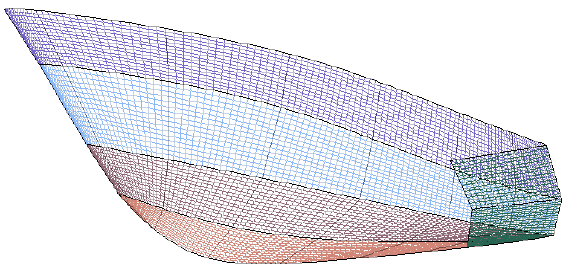
\includegraphics[width=0.5\textwidth,natwidth=585,natheight=273]{developplates.png}
        \caption{}
        \label{fig:developplates}
\end{wrapfigure}

\subsection{Develop plates.} \label{develop-plates}
All layers which are marked as developable in the layer properties
dialog are unfolded onto flat plates (a process also called
developing). If the model contains no developable layers then this
option appears disabled. Both sides of the ship are unfolded. A window
then appears showing the unfolded plates. It is best to assign each
strake or part of the hull to a different layer. Then each layer will
have its own unfolding. If a layer consists of multiple separate
parts, each part again will have its own unfolding. The unfolded
panels can be moved by dragging them with the mouse.  Buttons on the
toolbar at the top of the window can be used to rotate the currently
selected item.  The rotation angle of each panel may also be entered
manually. Zooming and panning can be done exactly as in the viewports
used for modeling the ship. Interior edges and any present
intersection curves are also drawn on the unfolded panels, and can be
switched on or off as desired. The initial settings for these options
are the same as those for the entire model. So if the stations are
turned off in the hullform-viewports, they will not show in the
developed surfaces window either, until they are turned on again.  The
viewport be can saved as a bitmap, but the visible parts can also be
exported to a .dxf file or sent directly to the printer/plotter. The
coordinates forming the boundary of each part can be exported to n
ASCII text file.

On the right of the window a list is visible, showing all unfolded
parts. By clicking on the checkboxes each part can be made visible or
invisible. At the top some crucial information about the developments
is shown. After the plates have been unfolded to 2D, ShipCAD compares
the length of the unfolded interior edges to the length of these edges
in 3D. If this length is smaller then the edges were compressed (drawn
in blue). If the unfolded edges are longer then these edges were
stretched (drawn in red). The min. error shown at the top is the
largest compression error that occurred (in world space dimensions, so
meters or feet). The max. error is the largest amount of stress of an
edge. Compressed or stretched edges may be visualized by turning both
the visibility of interior edges and highlighting of compressed edges
on. The difference in area between the 3D surface and the unfolded
surface is also shown. Below the displayed edges the number of
iterations it took to unfold the selected panel is shown. ShipCAD
makes up to 25 developments of each panel and uses the one with the
smallest overall error as the final one. Generally surfaces that are
truly developable are unfolded in 1 iteration, and have min. and
max. errors of 0.0. Surfaces that are not exactly developable can in
most cases still be unfolded but might have significant errors due to
the fact that the surface is curved in two directions. Think of it as
the top half of a sphere, you can not press this surface down to a
flat surface without stretching or compressing certain areas, unless
you make some cuts of course.  So it's \textbf{very important} to check these
errors when you actually want to use the unfolded plates for
construction purposes!

There are also two input fields to adapt the grid spacing. The grid
can be turned on and off from the toolbar. Each intersection of a grid
line and an unfolded panel has a number next to it indicating the
coordinate of that intersection.  The two panels that are created from
layers that border the centerplane of the hull and are completely
flat, such as for example a flat transom or bottom, are merged into 1
unfolded panel.

\begin{wrapfigure}{r}{0.5\textwidth}
        \centering
        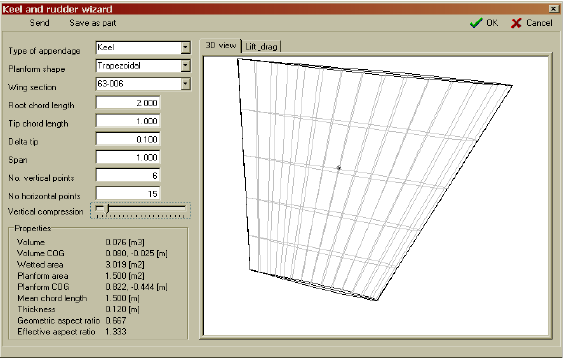
\includegraphics[width=0.5\textwidth,natwidth=566,natheight=360]{keelandrudder.png}
        \caption{}
        \label{fig:keelandrudder}
\end{wrapfigure}

\subsection{Keel and rudder wizard.}
The keel and rudder wizard enables you to quickly define a keel or
rudder with a predefined planform. You can select the desired
wingsection from a list of standard NACA sections. The keel or rudder
is show in 3D along with it basic properties such as aspect ratio,
volume, center of buoyancy etc.  Once the keel or rudder is complete
it can be exported in two ways. Using the “send” button it is inserted
at the current ShipCAD model at the origin. Using the “save as part”
button it can be saved to disc as a ShipCAD part which can be imported
in other designs. The lift/drag tab shows an estimation for the lift
and drag curves.

\subsection{Import markers.}
Markers are curves that can be added to the model as a reference. For
example the offsets of another design can be imported as markers. Then
intersection curves can be specified at the same locations in
ShipCAD. If the intersection curves coincide with the markers both
hulls are exactly the same. At the moment the only way to add markers
is by importing them from a textfile. The file format of this file is
exactly the same as as described in \ref{import-surface} Surface and
\ref{import-chines} Importing
chines.  The only difference is that the integer value on the first
line of the file that indicates the units used in the file (imperial
or metric) is discarded here.

\subsection{Delete markers.}
This deletes all markers from the model. It speaks for itself that
this option is disabled if there are no markers added to the
model. (see also \ref{vis-markers} Markers).

\subsection{Add cylinder.}
This option lets you add a cylinder. You can specify the startpoint,
endpoint, radius and number of points in the dialog that appears. The
points are calculated in such a way that the resulting surface has the
required properties, even though the points are located outside the
cylinder. The minimum number of points that can be used to form the
cylindrical shape is 4, however 6 or more is recommended. You can use
the cylinder for example to add a bow thruster to your model.

\pagebreak

\section{Transform.}
The first following 4 transformation operations described in this chapter are intended to be used on
a selection. There are two different ways to create such a selection.

\begin{enumerate}

\item Select the items yourself with the mouse

\item Select nothing. As soon as one of the commands below is chosen, and there is no
selection yet, the program shows a dialog from which you can select entire layers. Then the
operation is performed on the layers that you have selected.

\end{enumerate}

\subsection{Scale.} \label{scale}
Scales (part of) the model. For this operation the program assembles
all selected points, but also all the points that belong to edges and
faces that are selected. If nothing is selected, a dialog is presented
to the user from which entire layers can be selected. If the checkbox
at the bottom of the dialog is checked (the one saying: “include
points that are shared with unselected layers”) then a point is
selected automatically if \underline{\textit{at least}} one attached face belongs to a
selected layer. If the checkbox is not checked, then a point is
selected automatically when \underline{\textit{all}} the faces around it belong to selected
layer(s). If everything is selected, then not only is the hull scaled,
but mainparticulars, stations, buttocks and waterlines too.

\subsection{Move.}
Moves (part of) the model. Works on points extracted from a selection,
as described in \ref{scale} Scale.

\subsection{Rotate.}
Rotates (part of) the model. Works on points extracted from a
selection, as described in \ref{scale} Scale.

\begin{wrapfigure}{r}{0.3\textwidth}
        \centering
        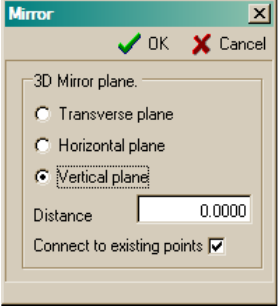
\includegraphics[width=0.3\textwidth,natwidth=279,natheight=308]{mirrordialog.png}
        \caption{}
        \label{fig:mirrordialog}
\end{wrapfigure}

\subsection{Mirror.}
In contrast to the previous transformation commands is this one based
on selected faces, not points. First select all the faces you want to
mirror (see the chapter about viewports for special selecting
options). Then use the mirror option to create a mirrored copy of the
selected faces. The mirror plane can be either transverse (YZ plane),
horizontal (XY plane) or vertical (XZ plane). The distance of the
mirror plane to the origin must be specified in the distance field.
The checkbox at the bottom of the form tells the program if the
mirrored points should be connected to already existing points or not.

\begin{wrapfigure}{r}{0.3\textwidth}
        \centering
        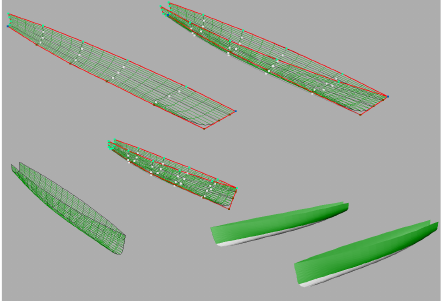
\includegraphics[width=0.3\textwidth,natwidth=443,natheight=303]{mirrorcatamaran.png}
        \caption{}
        \label{fig:mirrorcatamaran}
\end{wrapfigure}

As an example the image to the right shows the process of creating a
catamaran. The catamaran at first is modeled as a symmetrical monohull
(top left). To convert it to a proper catamaran the mirror option is
used. All faces of the (at this stage still a) monohull are selected
and mirrored in the centerplane of the hull (vertical plane, distance
= 0.0). This way a symmetrical monohull is obtained (top right). This
is finally moved in the positive y-direction with the \textit{move} command as
described in the paragraph above. If the visibility setting of the
program is set to show both sides of the design (in this case both
hulls) the final shape of the catamaran appears (bottom left and
bottom right)

\subsection{Lackenby.}
The hullform method developed by Lackenby is used to transform the
hull to match a desired displacement or longitudinal center of
buoyancy while maintaining fairness of your design. This is done by
shifting controlpoints in the longitudinal direction. So the overall
length of the design will be different after the transformation. The
dialog looks as follows:

\begin{figure}[h]
        \centering
        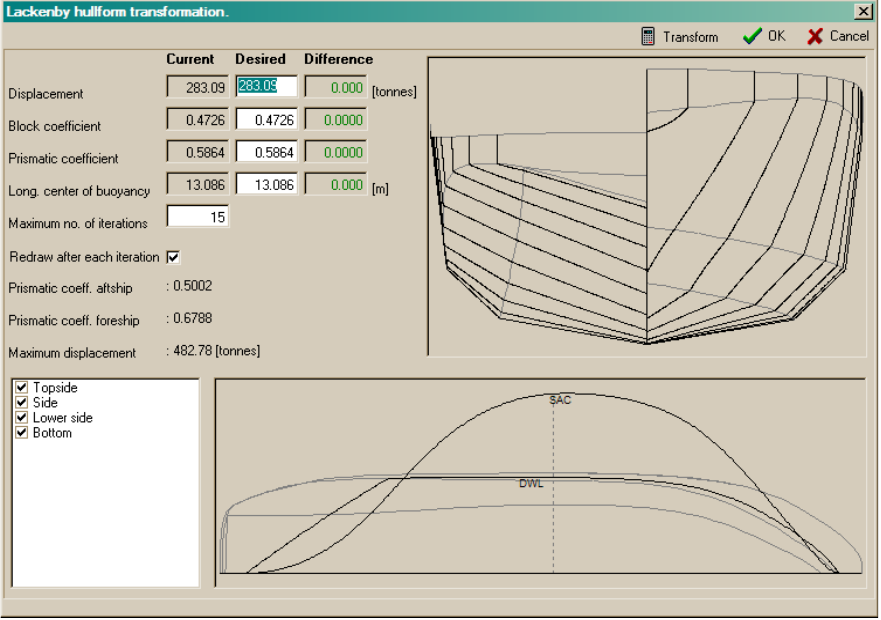
\includegraphics[width=15cm,natwidth=881,natheight=620]{lackenbydialog.png}
        \caption{}
        \label{fig:lackenby}
\end{figure}

The input fields to the left are divided in 3 columns. The left column
shows the current values as calculated from the model. The middle
column shows the desired values which can be modified by the user. The
right column shows the difference between the current and desired
values. The left and right column are updated after each iteration so
the progress can be monitored.

Below these 3 columns the maximum number of iterations that may be
performed can be modified.  The default is 15, but sometimes more
iterations are needed to obtain the desired result. This is specially
true when a design has a high prismatic coefficient in the aftship,
such as planing motorcraft, or when the midship location is far from
the usual place at 0.5*Length.

The checkbox below that ensures that all windows of the program are
updated after each iteration, so the progress can be monitored in 3D.

To the right the bodyplan of the original hull is displayed in
black. If the transformation was successful then the new bodyplan is
displayed in red dashed lines on top of the original bodyplan.

At the bottom of the dialog the original sectional area curve and
design waterline are displayed, also in black. Again the new sectional
area curve and design waterline are displayed on top of these if the
transformation was successful. The dark gray dashed line is the
location of the midship section as defined by the user in the project
settings. Important to know is that in contrast to the hydrostatics
calculated elsewhere in the program here it is calculated using
ordinates, and not surface panels. This can cause a slight difference
between the displacement shown here and calculated elsewhere. A total
of 82 ordinates is used to calculate the sectional area curve and
hydrostatics, 41 for the aftship and 41 for the foreship.

Finally at the bottom-left corner all layers of the model are
shown. The transformation is only applied to the layers that have a
checkmark next to them. As stated previously the transformation
consists of shifting controlpoints longitudinally, so the location of
for example a keel, centerboard or cabin is also likely to change. By
removing the checkmark layers containing such items remain unchanged,
but it may result in a distorted or unfair model if the model was
excessively changed.

\begin{figure}[h]
        \centering
        \includegraphics[width=15cm,natwidth=880,natheight=626]{lackenbydialog-2.png}
        \caption{}
        \label{fig:lackenby-2}
\end{figure}

Here the result is shown after transforming the blockcoefficient from
0.4726 to 0.5200. The new lines and sectional area curve are displayed
on top of the original lines.

\pagebreak

\section{Calculations.}

\begin{wrapfigure}{r}{0.3\textwidth}
        \centering
        \includegraphics[width=0.3\textwidth,natwidth=316,natheight=405]{intersectionsdialog.png}
        \caption{}
        \label{fig:intersection}
\end{wrapfigure}

\subsection{intersection curves.}
intersection curves such as stations, buttocks, waterlines and
diagonals are calculated from the model. Only their location needs to
be specified. Diagonals are always at an angle of 45 degrees to the
center plane. Each time the model is changed, the calculated
intersection curves are destroyed. They are rebuild as soon as they
need to be exported or drawn to the screen. The buttons on the toolbar
let you switch to which type of intersection you want to add or
delete. You can add one intersection at a time by selecting the +1
option in the menu. A dialog is displayed asking for the location of
the intersection. It is also possible to add a whole range at once by
selecting the +N option. Only the spacing between successive
intersection curves needs to be specified. The program starts at the
origin (x=0, y=0 or z=0, depending on the type of intersection) and
keeps adding intersection curves in positive and negative direction
until the extents of the model is reached. The intersection curves
appear in an increasing order of their distance. To delete an
intersection, just select it and press the \textit{delete} key on your
keyboard.

\begin{wrapfigure}{l}{0.5\textwidth}
        \centering
        \includegraphics[width=0.5\textwidth,natwidth=516,natheight=326]{curvaturevisibility.png}
        \caption{}
        \label{fig:curvaturevis}
\end{wrapfigure}

\begin{figure}[h]
        \centering
        \includegraphics[width=15cm,natwidth=942,natheight=335]{curvaturevisibility-2.png}
        \caption{}
        \label{fig:curvaturevis2}
\end{figure}

The checkbox displayed to the left of each intersection indicates if
the curvature plot of that specific intersection curve must be
plotted. (see curvature visibility). Due to the scale and nature of
the computer screen it is in almost any case impossible to determine
if a curve is fair. To overcome this a curvature plot is often
drawn. A curvature plot means that in a large number of points of a
curve the curvature is calculated and plotted perpendicular to the
curve ( the purple line). Since the curvature can be positive as well
as negative, the plot can swap from one side of the curve to the other
(see the image left). Where the plot intersects the curve the
curvature is zero. So in areas of a curve where the curvature is zero
(straight line segments), both curves are on top of each other. At a
knuckle point on the other hand the curvature is very high and can go
to infinity. So the higher the absolute value of the curvature, the
further the curvature plot is drawn away from the curve. Smooth curves
are characterized by curvature plots with no unexpected humps or
hollows, the curvature must change gradually as is the case with the
waterline below. The scale of the curvature plot can be decreased by
pressing the F9 key and increased by pressing the F10 key. Make sure
that the curvature visibility is also turned on!

\subsection{Design hydrostatics.} \label{design-hydrostatics}
A simple hydrostatic calculation is performed of the ship at the
design draft, as specified in the project settings. Some important
coefficients, such as blockcoefficient, are calculated twice. Once
using the length and beam as specified in the project settings, and
once using the actual length and beam at the waterline. Finally the
surface area and center of gravity of each layer is shown. These
properties are calculated for both sides of the ship and may be used
for example to estimate the weight of the hull.

If imperial units are used, the displacement is given in longtons (1
longton equals 2240 lbs).

\begin{figure}[h]
        \centering
        \includegraphics[width=15cm,natwidth=655,natheight=472]{hydrostaticsdialog.png}
        \caption{}
        \label{fig:hydrostaticsd}
\end{figure}

\subsection{Hydrostatics.}
This option is used to perform hydrostatic calculations at a range of
drafts. A trim may also be specified. The results can be saved to a
textfile.

\subsection{Cross curves.}
Stability calculations are provided in the form of cross curves. For a
number of heeling angles and displacements KN sin(ø) is calculated and
presented in a graph and table. If only one displacement is provided
the KN sin(ø) curve is displayed. If multiple displacements are
provided the graph shows the standard cross curves. The calculated
data can be printed or saved to a textfile.

\begin{figure}[h]
        \centering
        \includegraphics[width=10cm,natwidth=662,natheight=454]{crosscurvesdialog.png}
        \caption{}
        \label{fig:crosscurves}
\end{figure}

\subsection{Resistance calculations.}

\begin{wrapfigure}{r}{0.5\textwidth}
        \centering
        \includegraphics[width=0.5\textwidth,natwidth=672,natheight=408]{delftdialog.png}
        \caption{}
        \label{fig:delft}
\end{wrapfigure}

\subsubsection{Delft series.}
The Delft series resistance calculation is a method that is intended
for fin-keeled yachts. It's a statistical method based upon a whole
series of models that are tested over the years in the towing tank of
the Delft University of Technology. The calculation is restricted to
run only if the parameters of the model are in the same range as those
of the tested models.  These ranges are:

\begin{itemize}
  \item Lwl/Bwl [2.76 - 5.00]
  \item Bwl/Thull [2.46 - 19.32]
  \item Lwl/Displ\^0.333 [4.34 – 8.50]
  \item LCB (in \% of Lwl) [-6.0 – 0.0]
  \item Cp [0.52 – 0.60]
\end{itemize}

If there are no lines displayed in the graph to the right, then it's safe to assume that at least one of
the parameters is out of range. You can switch to the results tab to check the details.
There are two different ways to use the module:

\begin{itemize}

\item Fill in all the data manually. You don't even need a hull to do this. Each time a modification is
made everything is recalculated and updated.

\item Let the program calculate the hydrostatic values that are needed by clicking on the checkbox that
says: “Extract data from current hull”. Only two input fields
concerning the hull data are enabled in this mode. One is for the
draft of the hull alone, the other for the total draft of the hull
including the keel. This last draft is used when the hydrostatic
values are calculated, assuming you have indeed attached a keel at the
bottom of the hull. If this is not the case, then fill in the draft of
the hull alone as if it was the total draft including the keel. As all
data has been calculated by the program then disable the “extract from
hull” checkbox, and set the correct drafts in the two edit fields and
continue as normal.

\end{itemize}

All data used for the resistance calculation is stored with the model.

\subsubsection{KAPER.}
The KAPER resistance method is intended for canoes and kayaks. It was
originally developed by John Winters, a naval architect now
specializing in designing canoes and kayaks. (See
\url{http://www.greenval.com/jwinters.html}) It is based on statistical data obtained by model tests. His
method is later extended by Matt Broze to higher speed/length ratios
and to incorporate more variables into the equations. This extended
version is available in the form of an Excel spreadsheet
from \url{http://www.marinerkayaks.com/mkhtml/downloads.htm}. However
while implementing this method in ShipCAD two serious discontinuities
showed up in the curve of residual resistance.  These consist of a
sudden drop in resistance of about 10\% at speed/length ratios of 1.4
and 1.6 and are the result of a correction implemented by Matt. After
careful consideration the decision was made to only allow calculations
up to a speed/length ratio of 1.4 in order not to give the user a
false sense of security. It also restricts the method to stay within
the range of parameters of the actually tested hulls.

\begin{wrapfigure}{r}{0.5\textwidth}
        \centering
        \includegraphics[width=0.5\textwidth,natwidth=536,natheight=384]{kaperdialog.png}
        \caption{}
        \label{fig:kaper}
\end{wrapfigure}

Basically there are two ways to use the KAPER resistance method. The
easiest way is to open it with a design in memory. In that case the
checkbox saying “extract data from the current hull” is enabled and
may be checked. If it is checked all input fields, except those for
the draft and submerged transom ratio, are disabled.  When the draft
is changed the program calculates the appropriate hydrostatics
corresponding to that draft and the resistance data is updated. The
other way is by removing the check from the checkbox. In that case you
can specify (or modify after most values have been automatically
calculated) all input values manually.

After each modification the resistance is recalculated. You can see
the data either graphically on the first tab page or numerically on
the second tab page. When no data is visible the input data is out of
range. The range of valid parameters is:

\begin{itemize}

\item Prismatic coefficient 0.48-0.64

\item Submerged transom ratio 0.0-0.04

\item None of the other variables other than the waterline entrance angle me be zero.
The graph displays 4 resistance curves. The first three are for
frictional resistance, residual resistance and the total
resistance. The fourth line is showing the total resistance according
to Spilman. The residual resistance in this case is a very simple
formula based only upon the speed/length ratio of the design and is
included to give the user a point of reference.

\end{itemize}

All data entered in the input fields of this resistance method is also stored in the ShipCAD file.

\pagebreak

\begin{wrapfigure}{r}{0.4\textwidth}
        \centering
        \includegraphics[width=0.4\textwidth,natwidth=579,natheight=234]{backgroundimage-1.png}
        \caption{}
        \label{fig:backgroundimage1}
\end{wrapfigure}

\section{Background images.}
ShipCAD has the ability to show images on the background of your
model. This functionality is particularly convenient if you have an
existing linesplan on paper and want to recreate the lines in
ShipCAD. You can load a maximum of three images. Each of these images
is assigned to a view (profile, plan or bodyplan view). You can not
assign an image to the perspective view. All options related to
background images are located in the popup-menu that appears when you
press the right mouse button in a viewport. When using background
images pay special attention to make sure that all horizontal and
vertical lines on the images are truly horizontal or vertical.

\subsection{Visible.}
Once you have assigned an image to for example the profile view, it
will be shown in all viewports showing the profile view on the
model. By changing the \textit{visible property} you can hide the image from a
particular viewport.

\subsection{Clear.}
Using the clear command removes the image not only from the current
viewport but also from all other viewport. It is entirely removed from
the ShipCAD model.

\subsection{Load.}
Imports a background image. ShipCAD only reads \textit{bmp}
and \textit{jpg} images. For performance reasons make sure that the
images you are going to use are not too big. After having imported an
image you must set the origin to make sure it is displayed at the
right location. You also have to set the scale of the image to math
the size of your model.

\subsection{Save.}
Exports the background image to a file.

\subsection{Origin.}
If you use this option a special cursor appears. Once you click on a
spot in the active viewport that part of the image will be moved to
the origin of the current viewport. It does not necessarily have to be
a point within the actual background image, it may also be located
outside the image.

\subsection{Set scale.}
Make sure you set the scale of an imported image before opening another image. ShipCAD
assigns the same scale of the previously imported image to the freshly imported one. This is
particularly useful if you have multiple images imported from the same linesplan. When executing
this option the user is required to click on a point within the actual image of which the location is
known. The program uses the same scale for both the horizontal and vertical direction.

\begin{wrapfigure}{r}{0.5\textwidth}
        \centering
        \includegraphics[width=0.5\textwidth,natwidth=581,natheight=236]{backgroundimage-2.png}
        \caption{}
        \label{fig:backgroundimage2}
\end{wrapfigure}

\subsection{Transparent color.}
Often background images are in black and white. Having a huge white
area on your viewport can sometimes be distracting. By setting white
as the transparent color the program does not draw the white areas. So
only the black lines are draw on your screen. You can select the
transparent color by clicking on an area of the background image that
has the color you want to hide. If you click on a point that lies
outside the area of the background image transparency is disabled
again.

\begin{wrapfigure}{r}{0.5\textwidth}
        \centering
        \includegraphics[width=0.5\textwidth,natwidth=578,natheight=253]{backgroundimage-3.png}
        \caption{}
        \label{fig:backgroundimage3}
\end{wrapfigure}

\subsection{Tolerance.}
Sometimes images that look black and white
have a lot of colors in between. This is
particularly the case where some quality has
been lost due to compression, as is the case
with \textit{jpg} images. When white is the designated
transparent color and is filtered out, a lot of
``almost white'' pixels remain. By increasing the
tolerance these pixels can be filtered out by the
program too.

\subsection{Blending.}
If even after all the measures above the background image is till too
dominant, it can be blended with the viewport color. This way it
dissolves in the background and the geometry of you ShipCAD model is
still clearly visible.

\pagebreak

\section{Language support.} \label{language-support}
Current translations include:

\begin{itemize}

\item English

\item Dutch

\item German

\item French

\item Castellano

\item Suomi

\end{itemize}

Due to the fact that ShipCAD is still in development (new features
keep being added) and that the translations are created and maintained
by ShipCAD users, it is likely that the translation files are not
completely in sync with the most recent English.ini file. After each
official release the translation files have to be updated again. These
update files are then included in the next release of ShipCAD.

\subsection{Creating translations.}
All the text strings used on the forms are placed into a single .ini
file. The original file is called English.ini and can be found in the
Languages subdirectory. This is a simple textfile containing the
information of all forms where each form has it own section that
begins with the name of the form enclose by two square brackets, for
example: \textit{[TMainform]}. Each line after that has the following syntax:
\begin{verbatim}
TMainForm.LoadFile.Hint=Open a new file.
\end{verbatim}
This line can be split into two parts. The part left of the = sign
tells the program where the text should be placed, in this case it is
the hint that appears when the mouse hovers above the toolbar button
used to open a file. The part to the right of the = sign is the actual
text. When modifying the file make sure the = sign is not removed. You
can translate the file either with a ASCII text editor such as notepad
or use the special tool that can be downloaded from the ShipCAD
homepage. If you decide to make a translation, make sure you give the
file the name of the language you are translating into, as this is the
text that is displayed in the list with available languages in the
preferences dialog. New language files can be sent to
info@freeship.org so they can be included in the next release of
ShipCAD.

\pagebreak

\section{GNU General Public License.}

The GNU General Public License (GPL)
Version 2, June 1991
Copyright (C) 1989, 1991 Free Software Foundation, Inc.
59 Temple Place, Suite 330, Boston, MA 02111-1307 USA
Everyone is permitted to copy and distribute verbatim copies of this license document, but changing
it is not allowed.
Preamble
The licenses for most software are designed to take away your freedom to share and change it. By
contrast, the GNU General Public License is intended to guarantee your freedom to share and
change free software--to make sure the software is free for all its users. This General Public
License applies to most of the Free Software Foundation's software and to any other program
whose authors commit to using it. (Some other Free Software Foundation software is covered by
the GNU Library General Public License instead.) You can apply it to your programs, too.
When we speak of free software, we are referring to freedom, not price. Our General Public
Licenses are designed to make sure that you have the freedom to distribute copies of free software
(and charge for this service if you wish), that you receive source code or can get it if you want it,
that you can change the software or use pieces of it in new free programs; and that you know you
can do these things.
To protect your rights, we need to make restrictions that forbid anyone to deny you these rights or to
ask you to surrender the rights. These restrictions translate to certain responsibilities for you if you
distribute copies of the software, or if you modify it.
For example, if you distribute copies of such a program, whether gratis or for a fee, you must give
the recipients all the rights that you have. You must make sure that they, too, receive or can get the
source code. And you must show them these terms so they know their rights.
We protect your rights with two steps:
1.2.copyright the software, and
offer you this license which gives you legal permission to copy, distribute and/or modify the
software.
Also, for each author's protection and ours, we want to make certain that everyone understands that
there is no warranty for this free software. If the software is modified by someone else and passed
on, we want its recipients to know that what they have is not the original, so that any problems
introduced by others will not reflect on the original authors' reputations.
Finally, any free program is threatened constantly by software patents. We wish to avoid the danger
that redistributors of a free program will individually obtain patent licenses, in effect making the
program proprietary. To prevent this, we have made it clear that any patent must be licensed for
everyone's free use or not licensed at all.
The precise terms and conditions for copying, distribution and modification follow.
Terms and conditions for copying, distribution and modification.
1.2.3.This License applies to any program or other work which contains a notice placed by the
copyright holder saying it may be distributed under the terms of this General Public License.
The "Program", below, refers to any such program or work, and a "work based on the
Program" means either the Program or any derivative work under copyright law: that is to
say, a work containing the Program or a portion of it, either verbatim or with modifications
and/or translated into another language. (Hereinafter, translation is included without
limitation in the term "modification".) Each licensee is addressed as "you". Activities other
than copying, distribution and modification are not covered by this License; they are outside
its scope. The act of running the Program is not restricted, and the output from the Program
is covered only if its contents constitute a work based on the Program (independent of
having been made by running the Program). Whether that is true depends on what the
Program does.
You may copy and distribute verbatim copies of the Program's source code as you receive it,
in any medium, provided that you conspicuously and appropriately publish on each copy an
appropriate copyright notice and disclaimer of warranty; keep intact all the notices that refer
to this License and to the absence of any warranty; and give any other recipients of the
Program a copy of this License along with the Program. You may charge a fee for the
physical act of transferring a copy, and you may at your option offer warranty protection in
exchange for a fee.
You may modify your copy or copies of the Program or any portion of it, thus forming a work
based on the Program, and copy and distribute such modifications or work under the terms
of Section 1 above, provided that you also meet all of these conditions:
a) You must cause the modified files to carry prominent notices stating that you
changed the files and the date of any change.
b) You must cause any work that you distribute or publish, that in whole or in part
contains or is derived from the Program or any part thereof, to be licensed as a
whole at no charge to all third parties under the terms of this License.
c) If the modified program normally reads commands interactively when run, you must
cause it, when started running for such interactive use in the most ordinary way, to
print or display an announcement including an appropriate copyright notice and a
notice that there is no warranty (or else, saying that you provide a warranty) and that
users may redistribute the program under these conditions, and telling the user how
to view a copy of this License. (Exception: if the Program itself is interactive but does
not normally print such an announcement, your work based on the Program is not
required to print an announcement.)
4.5.These requirements apply to the modified work as a whole. If identifiable sections of that
work are not derived from the Program, and can be reasonably considered independent and
separate works in themselves, then this License, and its terms, do not apply to those
sections when you distribute them as separate works. But when you distribute the same
sections as part of a whole which is a work based on the Program, the distribution of the
whole must be on the terms of this License, whose permissions for other licensees extend to
the entire whole, and thus to each and every part regardless of who wrote it. Thus, it is not
the intent of this section to claim rights or contest your rights to work written entirely by you;
rather, the intent is to exercise the right to control the distribution of derivative or collective
works based on the Program. In addition, mere aggregation of another work not based on
the Program with the Program (or with a work based on the Program) on a volume of a
storage or distribution medium does not bring the other work under the scope of this
License.
You may copy and distribute the Program (or a work based on it, under Section 3) in object
code or executable form under the terms of Sections 2 and 3 above provided that you also
do one of the following:
a)b)c)Accompany it with the complete corresponding machine-readable source code, which
must be distributed under the terms of Sections 1 and 2 above on a medium
customarily used for software interchange; or,
Accompany it with a written offer, valid for at least three years, to give any third party,
for a charge no more than your cost of physically performing source distribution, a
complete machine-readable copy of the corresponding source code, to be distributed
under the terms of Sections 2 and 3 above on a medium customarily used for
software interchange; or,
Accompany it with the information you received as to the offer to distribute
corresponding source code. (This alternative is allowed only for noncommercial
distribution and only if you received the program in object code or executable form
with such an offer, in accord with Subsection b above.)
6.7.8.9.10.The source code for a work means the preferred form of the work for making modifications
to it. For an executable work, complete source code means all the source code for all
modules it contains, plus any associated interface definition files, plus the scripts used to
control compilation and installation of the executable. However, as a special exception, the
source code distributed need not include anything that is normally distributed (in either
source or binary form) with the major components (compiler, kernel, and so on) of the
operating system on which the executable runs, unless that component itself accompanies
the executable. If distribution of executable or object code is made by offering access to
copy from a designated place, then offering equivalent access to copy the source code from
the same place counts as distribution of the source code, even though third parties are not
compelled to copy the source along with the object code.
You may not copy, modify, sublicense, or distribute the Program except as expressly
provided under this License. Any attempt otherwise to copy, modify, sublicense or distribute
the Program is void, and will automatically terminate your rights under this License.
However, parties who have received copies, or rights, from you under this License will not
have their licenses terminated so long as such parties remain in full compliance.
You are not required to accept this License, since you have not signed it. However, nothing
else grants you permission to modify or distribute the Program or its derivative works. These
actions are prohibited by law if you do not accept this License. Therefore, by modifying or
distributing the Program (or any work based on the Program), you indicate your acceptance
of this License to do so, and all its terms and conditions for copying, distributing or modifying
the Program or works based on it.
Each time you redistribute the Program (or any work based on the Program), the recipient
automatically receives a license from the original licensor to copy, distribute or modify the
Program subject to these terms and conditions. You may not impose any further restrictions
on the recipients' exercise of the rights granted herein. You are not responsible for enforcing
compliance by third parties to this License.
If, as a consequence of a court judgment or allegation of patent infringement or for any other
reason (not limited to patent issues), conditions are imposed on you (whether by court order,
agreement or otherwise) that contradict the conditions of this License, they do not excuse
you from the conditions of this License. If you cannot distribute so as to satisfy
simultaneously your obligations under this License and any other pertinent obligations, then
as a consequence you may not distribute the Program at all. For example, if a patent license
would not permit royalty-free redistribution of the Program by all those who receive copies
directly or indirectly through you, then the only way you could satisfy both it and this License
would be to refrain entirely from distribution of the Program. If any portion of this section is
held invalid or unenforceable under any particular circumstance, the balance of the section is
intended to apply and the section as a whole is intended to apply in other circumstances. It is
not the purpose of this section to induce you to infringe any patents or other property right
claims or to contest validity of any such claims; this section has the sole purpose of
protecting the integrity of the free software distribution system, which is implemented by
public license practices. Many people have made generous contributions to the wide range
of software distributed through that system in reliance on consistent application of that
system; it is up to the author/donor to decide if he or she is willing to distribute software
through any other system and a licensee cannot impose that choice. This section is intended
to make thoroughly clear what is believed to be a consequence of the rest of this License.
11. If the distribution and/or use of the Program is restricted in certain countries either by
patents or by copyrighted interfaces, the original copyright holder who places the Program
under this License may add an explicit geographical distribution limitation excluding those
countries, so that distribution is permitted only in or among countries not thus excluded. In
such case, this License incorporates the limitation as if written in the body of this License.
12. The Free Software Foundation may publish revised and/or new versions of the General
Public License from time to time. Such new versions will be similar in spirit to the present
version, but may differ in detail to address new problems or concerns. Each version is given
a distinguishing version number. If the Program specifies a version number of this License
which applies to it and "any later version", you have the option of following the terms and
conditions either of that version or of any later version published by the Free Software
Foundation. If the Program does not specify a version number of this License, you may
choose any version ever published by the Free Software Foundation.
13. If you wish to incorporate parts of the Program into other free programs whose distribution
conditions are different, write to the author to ask for permission. For software which is
copyrighted by the Free Software Foundation, write to the Free Software Foundation; we
sometimes make exceptions for this. Our decision will be guided by the two goals of
preserving the free status of all derivatives of our free software and of promoting the sharing
and reuse of software generally.
NO WARRANTY
14. BECAUSE THE PROGRAM IS LICENSED FREE OF CHARGE, THERE IS NO
WARRANTY OR THE PROGRAM, TO THE EXTENT PERMITTED BY APPLICABLE LAW.
EXCEPT WHEN OTHERWISE STATED IN WRITING THE COPYRIGHT HOLDERS
AND/OR OTHER PARTIES PROVIDE THE PROGRAM "AS IS" WITHOUT WARRANTY OF
ANY KIND, EITHER EXPRESSED OR IMPLIED, INCLUDING, BUT NOT LIMITED TO, THE
IMPLIED WARRANTIES OF MERCHANTABILITY AND FITNESS FOR A PARTICULAR
PURPOSE. THE ENTIRE RISK AS TO THE QUALITY AND PERFORMANCE OF THE
PROGRAM IS WITH YOU. SHOULD THE PROGRAM PROVE DEFECTIVE, YOU ASSUME
THE COST OF ALL NECESSARY SERVICING, REPAIR OR CORRECTION.
15. IN NO EVENT UNLESS REQUIRED BY APPLICABLE LAW OR AGREED TO IN WRITING
WILL ANY COPYRIGHT HOLDER, OR ANY OTHER PARTY WHO MAY MODIFY AND/OR
REDISTRIBUTE THE PROGRAM AS PERMITTED ABOVE, BE LIABLE TO YOU FOR
DAMAGES, INCLUDING ANY GENERAL, SPECIAL, INCIDENTAL OR CONSEQUENTIAL
DAMAGES ARISING OUT OF THE USE OR INABILITY TO USE THE PROGRAM
(INCLUDING BUT NOT LIMITED TO LOSS OF DATA OR DATA BEING RENDERED
INACCURATE OR LOSSES SUSTAINED BY YOU OR THIRD PARTIES OR A FAILURE
OF THE PROGRAM TO OPERATE WITH ANY OTHER PROGRAMS), EVEN IF SUCH
HOLDER OR OTHER PARTY HAS BEEN ADVISED OF THE POSSIBILITY OF SUCH
DAMAGES.

\end{document}
